%\customlink{How_rocks_get_and_stay_magnetized}
\chapter{How rocks get and stay magnetized}
\label{sect:nrmintro}

\noindent
BACKGROUND:  read Widom  (2002), Chapter 1. \nocite{widom02}
\vskip 24pt

The key to the acquisition of magnetic remanence is magnetic anisotropy energy,  the dependence of  magnetic energy on  direction of magnetization within the crystal ( see Chapter 4).  It is magnetic anistotropy energy that  controls the probability of magnetic grains changing their moments from one easy direction to another.   Without it,
the magnetic moments of individual grains would swing freely and could not retain
a ``memory'' of the ancient field direction.   

Anisotropy energy controls relaxation time, a concept briefly introduced in Chapter 4 where  we defined it as a time constant for decay of the magnetization of an assemblage of magnetic grains when placed in a null field.  Equation~\ref{eq:MvT} predicted exponential decay with   relaxation time $\tau$ being the  time it takes for the initial magnetization to decay to $1/e$ of its initial value.     Relaxation time reflects the probability of magnetic moments jumping over  the anisotropy energy barrier between easy axes. 
Therefore, to preserve a record of an ancient geomagnetic field, 
there must be a way that  the relaxation time changes from short (such that the magnetization is in  equilibrium with the ambient geomagnetic field)
to long (such that the magnetization is ``frozen'', or blocked,  for geologically significant periods of time).  



Before we begin a more detailed look at the processes governing remanence acquisition, it is helpful to review briefly what is meant by
\index{equilibrium}
``equilibrium'' in physics and chemistry.  Eager students are encouraged to read the background material recommended in the ``BACKGROUND'' list at the beginning of the chapter.  In the following,  we will go through the bare bones of statistical mechanics necessary to understand natural remanence.


\section{The concept of dynamic equilibrium}
\index{equilibrium!dynamic}

We live in a world that is  in constant motion  down to the atomic level. The state of the things is constantly changing, but, looking at the big picture, things often seem to stay the same.  Imagine for a moment a grassy field full of sheep and  a fence running down the middle.  The sheep can jump over the fence at will to get flowers on the other side and occasionally they do so.   Over time, because the two sides of the fence  are pretty much the same, the same number of sheep jump over in both directions, so if you were to count sheep on either side, the numbers would stay about the same.



\begin{figure}[htb]
%\epsfxsize 10cm
%\centering \epsffile{EPSfiles/equilibrium.eps}
\centering  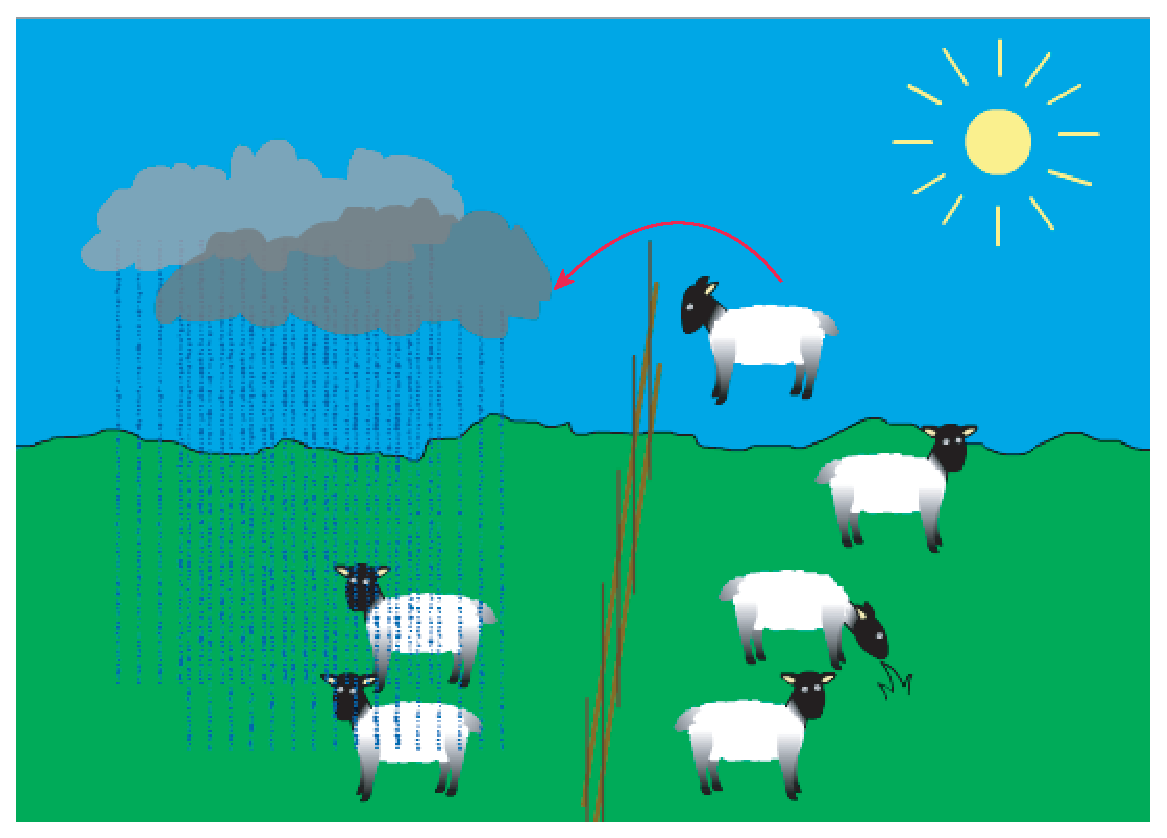
\includegraphics[width=10 cm]{EPSfiles/equilibrium.eps}
\caption{Illustration of dynamic equilibrium.  If conditions on either side of the fence are equally pleasant, an equal number of sheep will be on either side of the fence, despite the fact that sheep are constantly jumping over the fence.  If one side is preferable (sunny rather than rainy), there will tend to be more sheep on the nicer side.  [Drawing by Genevieve Tauxe modified from animation  available at: \newline \url{http://magician.ucsd.edu/Lab_tour/movs/equilibrium.mov}.]}
\label{fig:equilibrium}
\end{figure}

Now think about what would happen if it were raining on one side of the fence.   The sheep would jump more quickly back over the fence from the rainy side to the sunny side than the other way around. You might find that over time, there were more sheep on the sunny side than on the rainy side (see Figure~\ref{fig:equilibrium}).   If you are still awake after all this sheep counting, you have begun to understand the concept of dynamic equilibrium.



Returning to magnetism, a magnet with uniaxial anisotropy in the absence of a magnetic field will tend to be magnetized in one of several possible ``easy'' directions (see Chapter 4).  For the purpose of this discussion, let us consider the case of uniaxial anisotropy, in which there are only two easy directions in each magnetic grain.   In order to ``jump over the fence''  (the 
\index{anisotropy!energy}
anisotropy energy) and get from one easy axis to another, a magnetic particle must have thermal energy in excess of the anisotropy energy.  According to the 
\index{Boltzmann's!distribution law}
Boltzmann distribution law, the probability of a given particle having an energy $E$ is proportional to $e^{ -E/kT}$ where $kT$ is the 
\index{thermal energy}
thermal energy (see Chapter 4).   Therefore, it may be that at a certain time, a particular magnetic grain has enough thermal energy for the electronic spins to overcome the energy barrier and flip the sense of magnetization from one easy axis to another.  

If we had a collection of magnetized particles with some initial statistical alignment of moments giving a net remanence $M_o$, (more sheep on one side than the other),  the random ``fence jumping'' by magnetic moments from one easy axis to another over time will eventually lead to the case where there is no preference and the net  moment will have decayed to zero (although the individual grain moments remain at saturation).    This approach to 
\index{magnetization!equilibrium}
{\it equilibrium  magnetization} ($M_e$)  is the theoretical underpinning of Equation~\ref{eq:MvT} 
 (plotted in Figure~\ref{fig:neel}a) and is the essence of what is known as
 \index{N\'eel!theory}
  N\'eel Theory.
  
\begin{figure}[h!tb]
%\epsfxsize 14cm
%\centering \epsffile{EPSfiles/neel.eps}
\centering  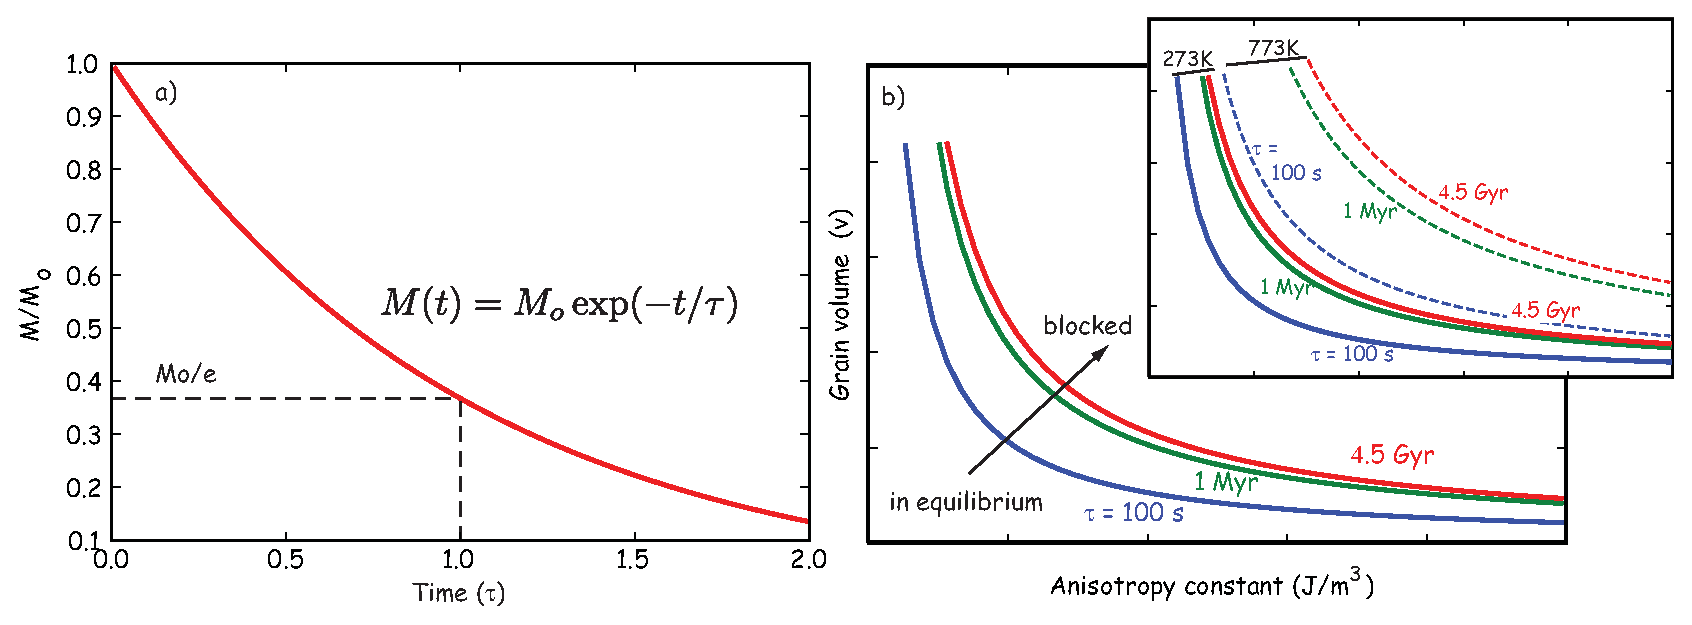
\includegraphics[width=14 cm]{EPSfiles/neel.eps}
\caption{ a) Magnetic relaxation in an assemblage of single domain ferromagnetic grains.  The initial magnetization  $M_o$ decays to $1\over e$ of its original strength in time $\tau$. b) Relaxation times of single domain grains on a plot of  grain
volume, $v$, against an anisotropy energy constant ($K$), for a  given temperature.  Grains with short relaxation times plot toward the lower left and are in equilibrium with the magnetic field (they are superparamagnetic). Grains with long relaxation times plot toward the upper right;  their moments are blocked, preserving the magnetization for geologically significant times.  Inset shows the effect of temperature on the relaxation time curves which move toward the right and up with increasing temperature, changing ``blocked'' remanences to unblocked ones.  }
\label{fig:neel}
\end{figure}
 


\section {Essential  N\'eel theory}


The theoretical basis for how ancient magnetic fields might be preserved was established over fifty years ago with the  work of Nobel prize winner  
\index{N\'eel, L.}
Louis N\'eel (1949, 1955). \nocite{neel49} \nocite{neel55}
In the introduction to this chapter, we suggested that the  mechanism which controls the approach to magnetic
\index{equilibrium!magnetic}
 equilibrium is   relaxation time.  In the sheep analogy this would be  the frequency of fence jumping. We defined relaxation time  by Equation~\ref{eq:tau} in  Chapter 4, sometimes called  the 
 \index{N\'eel!equation}
  {\it N\'eel equation},  which  relates  $\tau$ to volume $v$, the anisotropy constant ($K$) and  absolute temperature ($T$). 
     
 Relaxation time is controlled by the competition between anisotropy energy $Kv$ and thermal energy, so will be constant at a given temperature with constant $Kv$.  Iso-$\tau$s of equal relaxation time are curves in $v-K$ space. Figure~\ref{fig:neel}b shows the family of curves with $\tau$s ranging from $\sim$100 seconds to  the age of the Earth.     The inset to Figure~\ref{fig:neel}b illustrates the effect of temperature on the iso-$\tau$s,  which move up and to the right with increasing temperature.  This  behavior gives us a clue as to how a rise in temperature could change a  ``blocked'' remanence at 0$^{\circ}$C (273K) (one that is stable for long periods of time) to an unblocked  one.    In fact, Figure~\ref{fig:neel}b (and the inset) suggests two other ways of manipulating the approach to equilibrium besides temperature:  by changing the time span of observation  and by changing grain volume.  Each of these mechanisms represents a different mode of remanence acquisition  (thermal, viscous, and chemical remanences respectively).   Naturally acquired remanences are generally referred to as 
 \index{magnetization!remanent!natural}
{\it natural remanent magnetizations}  or NRMs.  In this chapter we will introduce these and other forms of NRM and how they are acquired.   We will also introduce useful unnatural remanences where appropriate.  
  
  
  
  
  
  
  In the ``sheep in the rain'' scenario, jumping over the fence into the sun would  occur more frequently  than jumping into the rain.  It is also true that the energy barrier for magnetic particles to flip into the direction of the applied field $\H$ requires less energy than to flip the other way, so relaxation time must also be a function of the applied field.    This tendency is reflected in the more general form of the N\'eel equation:

\begin{equation}
{\tau} = { { 1\over C} \exp { [Kv] \over [kT]}}{  \bigl[ 1 -  { H\over H_c}\bigr] ^2 }.
\label{eq:tau2}
\end{equation}

\noindent  
In this chapter we are concerned mainly with magnetic remanences acquired in the presence of the Earth's magnetic field, which is tiny compared to the coercivity of the minerals in question and so we can neglect the effect of $H$ on $\tau$ in  the next few sections.  

In Equation~\ref{eq:tau2},   the product $K v$ is an energy barrier to the rotation of $\m$ and we will call it  the
\index{energy!blocking}
{\it  blocking energy}.   High blocking energies will promote more stable magnetizations.    We  learned  in Chapter 4 that $K$ for uniaxial shape anisotropy, $K_u $, is related to the   
 \index{coercivity}
 coercivity $H_c$ (the field required to flip the magnetization)  by:
 
 $$H_c= {{2 K_u}\over{\mu_o M_s}},$$
 
 \noindent where $M_s$ is the saturation magnetization.  Substituting for $K_u$ in Equation~\ref{eq:tau} from Chapter 4  we get:

\begin{equation}
{\tau } =
{{1\over C} \exp {{[\mu_o H_c M_s v]}\over {[2kT]}}},
\label{eq:tau3}
\end{equation}

\noindent  where  $M_s$ is itself a  strong function of temperature (see, e.g., Figure~\ref{fig:curie} in Chapter 3).  
We can see from Equation~\ref{eq:tau3} that relaxation time is a function of  magnetization, as well as volume, coercivity and temperature, properties that we will return to later in the chapter and in future chapters through out the course.  

\begin{figure}[h!tb]
%\epsfxsize 8cm
%\centering \epsffile{EPSfiles/neel-vrm.eps}
\centering  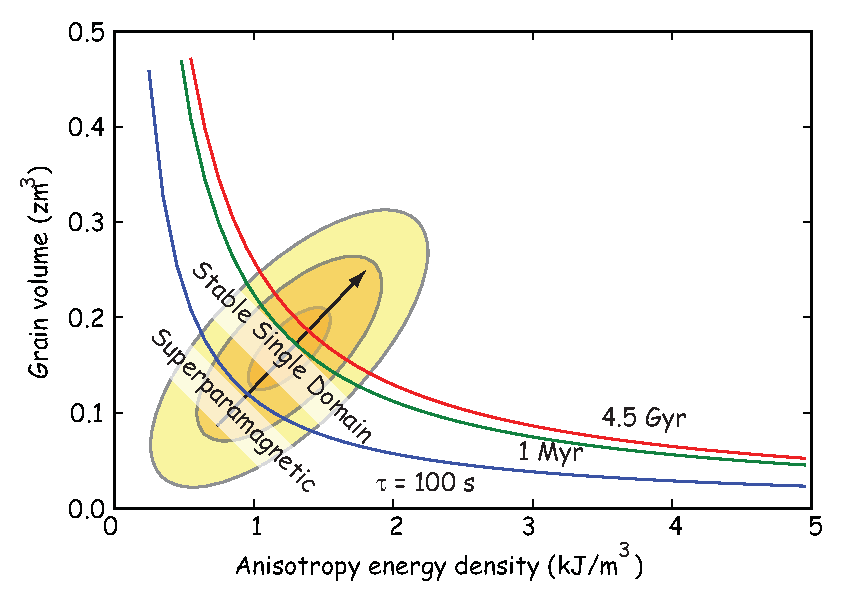
\includegraphics[width=8 cm]{EPSfiles/neel-vrm.eps}
\caption{Lines of equal blocking energy in plot of   grain
volume, $v$, against the anisotropy energy density, $K$. Lines of equal blocking energy (product $Kv$) are also lines of equal relaxation time, $\tau$, at a given temperature (here assumed to be room temperature).  Contours are for a hypothetical population of magnetic grains.  Grains with short $\tau$ plot toward the lower left. Grains with long $\tau$  plot toward the upper right; superparamagnetic grains with $\tau < 100$s  plot to the left or below the ``superparamagnetic line'' when $\tau \simeq$ 100s . Stable single domain grains
with $\tau > $100s plot above or to  right of  superparamagnetic line. }
\label{fig:neel-vrm}
\end{figure}



It is instructive to plot distributions of grains on the 
\index{diagrams!$v-K$}
$v-K$ diagrams as shown in Figure~\ref{fig:neel-vrm}b.    
By definition, superparamagnetic grains are those grains whose remanence relaxes quickly. A convenient
critical relaxation time,  for purposes of laboratory experiments may be taken as $\sim$100 s.  Effective paleomagnetic recorders must have relaxation times on the order of geological time. So it
might be more appropriate to choose $\tau$s of the age of the Earth (4.5 Gyr)  as the relevant relaxation for geological time scales. 




We will now consider various mechanisms by which rocks can become magnetized.  The first mechanism, 
 \index{magnetization!remanent!viscous}
viscous remanent magnetization,  is  simply a consequence of Equation ~\ref{eq:tau}  in Chapter 4 and Figure~\ref{fig:neel}a.    Later, we will explore the role of temperature and grain volume in blocking of thermal and chemical  remanences.    We will finish this chapter with other remanences which are either rare or non-existent in nature but are nonetheless useful in paleomagnetism.  


\section {Viscous remanent magnetization}
\label{sect:vrm}


 Placing a magnetic particle at an angle $\theta$ to an external magnetic field results in a magnetostatic energy $E_m$ of $-\m \cdot \B = -mB\cos \theta$, which is at a minimum when the moment is aligned with the field (see Chapters 1 and 5).      Given an arbitrary $\theta$, the difference in $E_m$ between the two easy directions is given by: 

\begin{equation}
\Delta E = 2(\m \cdot \B) = 2mB \cos \theta.
\label{eq:deltaE}
\end{equation}



Because of the energy of the applied field $E_m$, the energy necessary to flip the moment from a direction with a high angle to the external field to the other direction with a lower angle is less than the energy necessary to flip the other way around.   Therefore, a given particle will tend to spend more time with its moment at a favorable angle to the applied field than in the other direction.  
Moreover,  the 
\index{Boltzmann's!distribution law}
Boltzmann distribution law tells us that the longer we wait, the more likely it is  for a given magnetic grain to have the energy to overcome the barrier and flip its moment.   That is why over time the net magnetization of assemblages of magnetic particles  will tend to grow (or decay) to some \index{magnetization!equilibrium}
equilibrium magnetization $M_e$.  

We can visualize what happens in Figure~\ref{fig:neel-vrm}b.  Let us place an assemblage of magnetic grains with some initial magnetization $M_o$ in a magnetic field.   At a given time span of observation ($\tau$),  particles with that relaxation time are likely to have sufficient energy to overcome the energy barriers.   In a given assemblage of 
\index{blocking!energy}
 blocking energies (shown as the contours),  some grains will be tending toward equilibrium with the external field (those to the left and below the blocking energy line) while some will tend to remain fixed (those to the right of the line).  As the time span of observation increases,  the critical blocking energy line migrates  up and to the right (moving from 100 s, to 1 Myr,  and so on) and whatever initial magnetic state the population was in will be progressively re-magnetized in the external field.  


\begin{figure}[h!tb]
%\epsfxsize 14cm
%\centering \epsffile{EPSfiles/vrm1.eps}
\centering  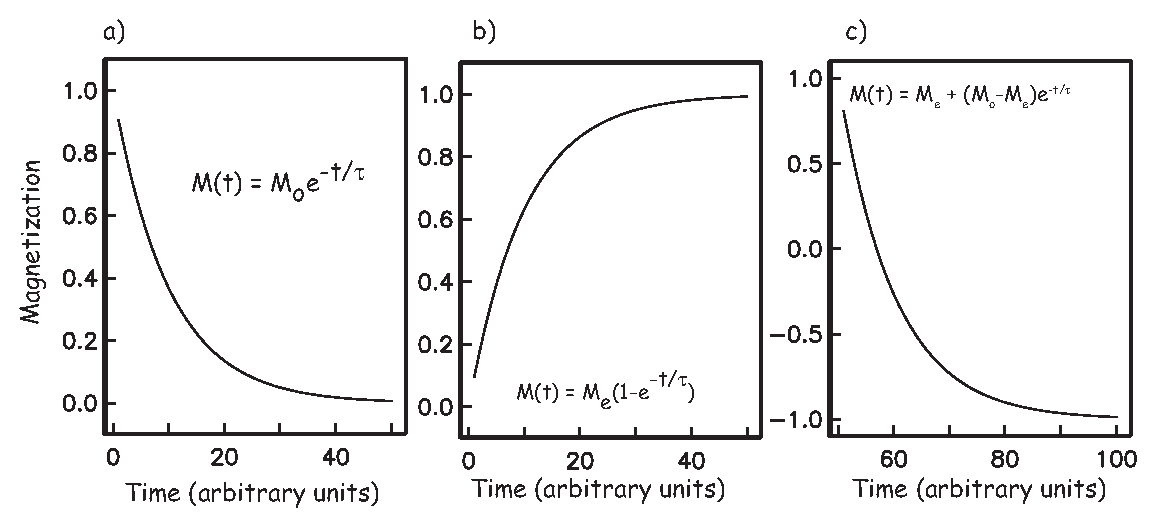
\includegraphics[width=14 cm]{EPSfiles/vrm1.eps}
\caption{Magnetization versus time for  a) Saturation remanence placed in zero field.   b) Zero initial magnetization placed in a field.  c) Magnetization placed in an antiparallel field.  }
\label{fig:vrm1}
\end{figure}
\eject

In Figure~\ref{fig:vrm1} we consider a few different  scenarios for $M_o$ and the applied field.  First,  the already familiar case when  a specimen with a net magnetization ($M_o$) is placed in zero external field; the magnetization will decay to zero as in Figure~\ref{fig:vrm1}a.  Conversely, if a specimen with zero initial remanence is put into a
magnetic field,
the magnetization $M(t)$ will grow to 
 $M_e$ by the complement of the decay equation:

\begin{equation}
M(t)=M_e(1-e^{-t/\tau}),
\label{eq:vgrow}
\end{equation}
 
\noindent as shown in Figure~\ref{fig:vrm1}b.  
The magnetization that is acquired in this isochemical, isothermal fashion is termed
 \index{magnetization!remanent!viscous}
{\it viscous remanent magnetization} or VRM and the equilibrium magnetization $M_e$ is a function of the external field $B$.

The general case, in which the initial magnetization of a  specimen is
nonzero and the 
\index{equilibrium!magnetization}
equilibrium magnetization is of arbitrary orientation to the initial remanence, the equation can  be written as:

\begin{equation}
\M(t)=\M_o + (\M_e-\M_o)(1-e^{-t/\tau}) = \M_e + (\M_o-\M_e)\cdot
e^{-t/\tau},
\label{eq:vrm}
\end{equation}

\noindent which grows (or decays) exponentially from $\M_o \rightarrow \M_e$ as
$t \rightarrow
\infty $. The rate is not only controlled by $\tau$,
but also  by the degree
to which the magnetization is out of equilibrium (see Figure~\ref{fig:vrm1}c). 

\begin{figure}[htb]
%\epsfxsize 14cm
%\centering \epsffile{EPSfiles/neel-trm.eps}
\centering  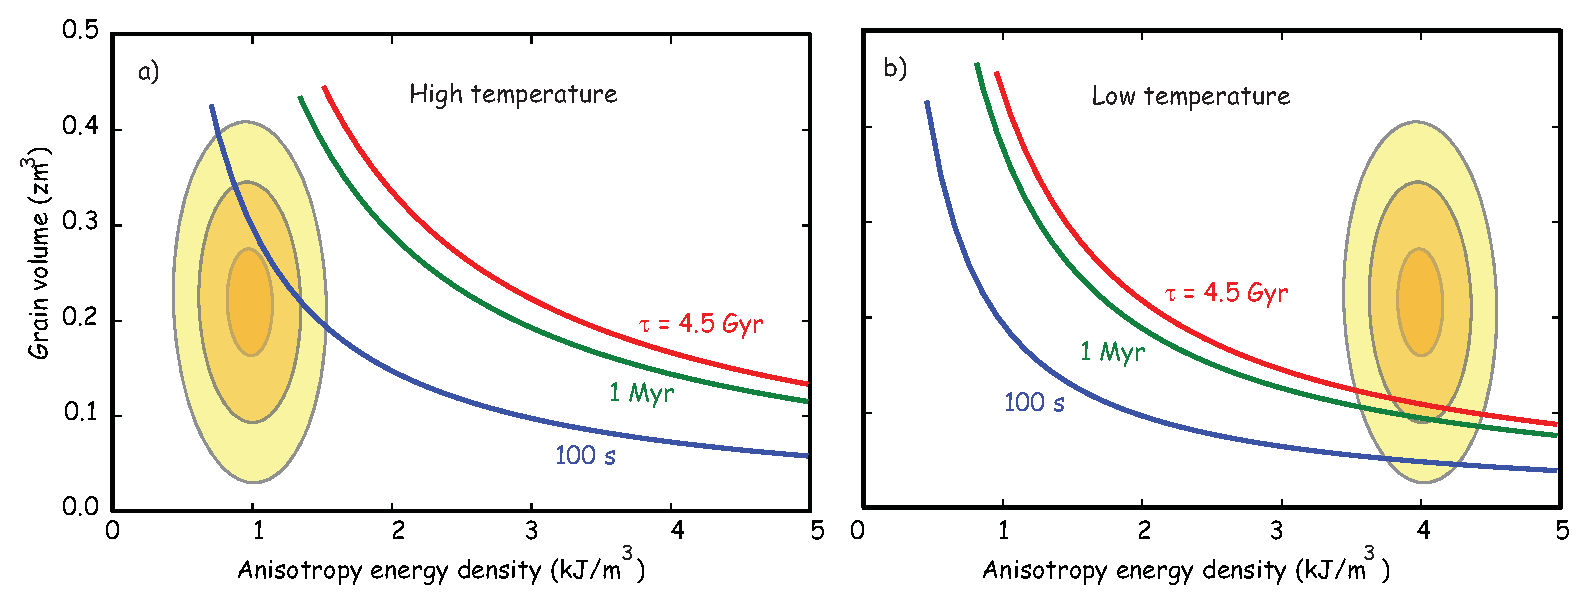
\includegraphics[width=14 cm]{EPSfiles/neel-trm.eps}
\caption{Migration of the relaxation times of a population of magnetic grains from a) low anisotropy energy at high temperature  to b) high anisotropy energy at lower temperatures and the resulting change in relaxation times.   The relaxation time curves also migrate up and to the right with lower thermal energy.   Any particle initially to the right or above the superparamagnetic line would acquire a TRM its anisotropy energy density  migrated across the line by cooling.  Note that the anisotropy energy density ($K$ from Chapter 4) itself is a function of temperature through its dependence on magnetization, so a given population of grains will change with changing temperature, migrating to the left with higher temperature as magnetization goes down .  }
\label{fig:trm-neel}
\end{figure}


Some temporally short data sets appear to follow the relation $M(t)\propto \log(t)$ and
\index{N\'eel, L.}
 N\'eel (1949, 1955)  suggested that VRM = S  log $t$.  Such a relationship
suggests infinite remanence as $t \rightarrow \infty $, so cannot be
true over a long period of time.
S log $t$  behavior can generally only be observed over a restricted
time interval and closely spaced, long-term observations do not show
linear  $\log(t)$-behavior, but are all curved in $\log(t)$ space.   When under-sampled, these time series can appear segmented, leading to interpretations of several quasi-linear features (multiple values of $S$), when in fact the time series are not linear at all.  



 VRM is a function of time and the relationship between the remanence vector and the applied field.  When the relaxation time is short (say a few hundred seconds), the magnetization is essentially in equilibrium with the applied magnetic field hence is superparamagnetic.  
  Because relaxation time  is also a strong function of temperature, VRM will grow more rapidly at higher temperature.    As noted in Chapter 4 there is a very sharply
defined range of temperatures over which $\tau $ increases from geologically
short to geologically long time scales.    In the next section, we consider the magnetization acquired by manipulating relaxation time by changing temperature: 
 \index{magnetization!remanent!thermal}
thermal remanent magnetization (TRM).    


\begin{figure}[h!tb]
%\epsfxsize 10cm
%\centering \epsffile{EPSfiles/tauT.eps}
\centering  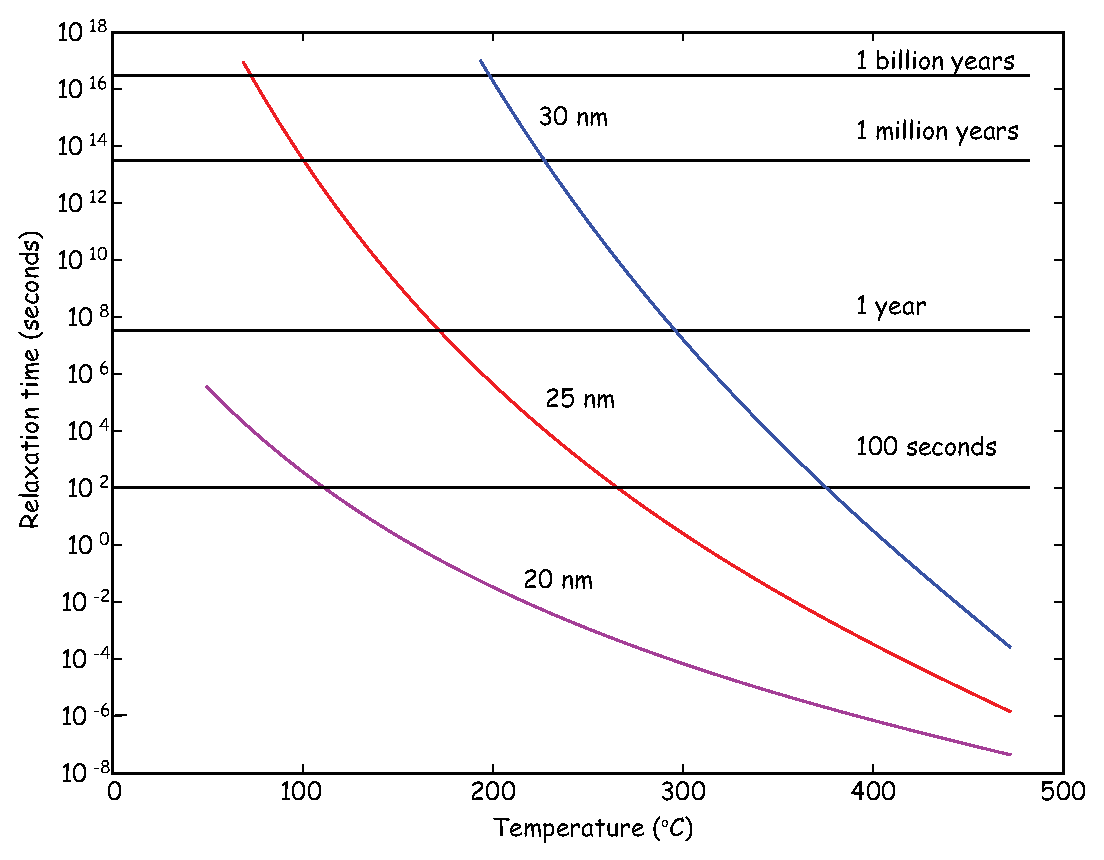
\includegraphics[width=10 cm]{EPSfiles/tauT.eps}
\caption{Variation of relaxation time versus temperature for magnetite ellipsoids of different widths (all with length to width ratios of 1.3:1).  }
\label{fig:tauT}
\end{figure}

 
\section {Thermal remanent magnetization}
\label{sect:trm}


The
\index{blocking!energy}
 $v-K$ diagram shown in Figure~\ref{fig:trm-neel} illustrates how TRM can be blocked.  In Figure~\ref{fig:trm-neel}a we have a population of magnetic grains with varying volumes and anisotropies.   Raising temperature works in two ways on these grains.  First,  the
 \index{relaxation time}
  relaxation time depends on thermal energy, so higher temperatures will result in lower blocking temperatures.  Second,  anisotropy energy depends on the square of magnetization (Chapter 4).  Elevated temperature reduces magnetization,   so  the anisotropy energy will be depressed  relative to lower temperatures.   In the diagram, this means that not only do the relaxation time curves move with changing temperature, but the anisotropy energies of the population of grains change as well.    This means that a population of grains that are superparamagnetic at high temperature (Figure~\ref{fig:trm-neel}a) could be ``blocked'' as cooling causes the grains to ``walk'' through the superparamagnetic threshold into a region of magnetic stability (Figure~\ref{fig:trm-neel}b).   



The key to 
\index{N\'eel!theory}
N\'eel theory is that very small changes in conditions (temperature, volume, anisotropy energy) can result in enormous changes in relaxation time.   In order to work out how relaxation time varies with temperature, we need to know how saturation magnetization varies with temperature.   We found  in Chapter 3 that calculating $M_s (T)$  exactly is a rather messy process.    If we take a reasonable value for   $\gamma$  in Equation~\ref{eq:MsT} from the data in Figure~\ref{fig:curie} in Chapter 3   or  $\gamma \simeq$ 0.38     and  $M_s$ = 480 mAm$^{-1}$ (from Chapter 6)  we can calculate the variation of relaxation time as a function of temperature for  elllipsoidal grains of various widths using Equation~\ref{eq:tau3} (see  Figure~\ref{fig:tauT}).  At room temperature, a 25 nm ellipsoid of magnetite (length to width ratio of 1.3:1)  would have a relaxation time of billions of years, while at 300$^{\circ}$C, the grain would be   superparamagnetic.  




The sharpness of the relationship between relaxation time and temperature allows us to define a  temperature  above which a grain is 
\index{superparamagnetism}
superparamagnetic and able to come into
\index{equilibrium!magnetic}
 magnetic equilibrium with an applied field and below which it is effectively blocked.  The temperature at which $\tau $ is
equal to a few hundred seconds  is defined as the 
\index{blocking!temperature}
{\it blocking temperature} or $T_b$.  At or above the blocking temperature, but  below the Curie
Temperature, a grain will be 
superparamagnetic.  Cooling  below $T_b$  increases 
the relaxation time sharply, so the magnetization is effectively blocked and the rock acquires a
 \index{magnetization!remanent!thermal}
 {\it thermal remanent magnetization} or TRM.

\begin{figure}[h!tb]
%\epsfxsize 14cm
%\centering \epsffile{EPSfiles/lava.eps}
\centering  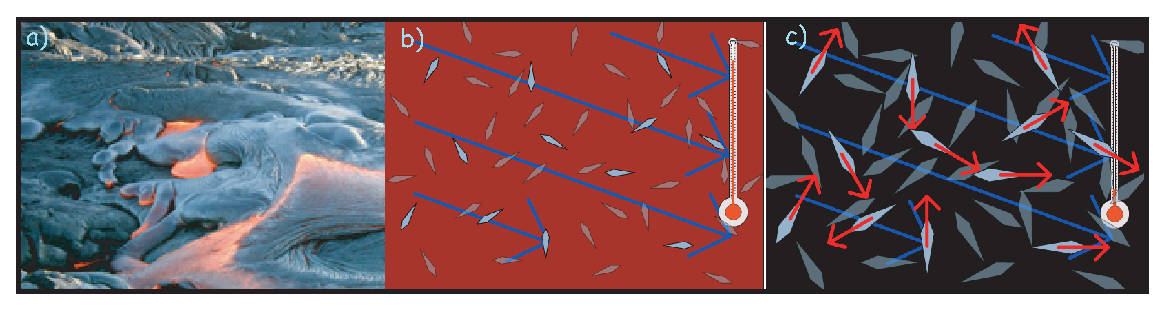
\includegraphics[width=14 cm]{EPSfiles/lava.eps}
\caption{a) 
Picture of lava flow courtesy of Daniel Staudigel.  b) While the lava is still well above the Curie temperature, crystals start to form, but are non-magnetic.  c) Below the Curie temperature but above the blocking temperature,  certain minerals become magnetic, but their moments continually flip among the easy axes with a statistical preference for the applied magnetic field.  As the lava cools down, the moments become fixed, preserving a thermal remanence.  [b) and c) modified from animation of Genevieve Tauxe available at:  \newline \url{http://magician.ucsd.edu/Lab_tour/movs/TRM.mov}.] [Figure from Tauxe and Yamazaki, 2007.]
 }
\label{fig:lava}
\end{figure}


Now let us put some of these concepts into practice.  
Consider a lava flow which has just been extruded (Figure~\ref{fig:lava}a).
Upon meeting the chilly air (or water),  molten lava  solidifies quickly into rock.  While the rock is above the 
\index{Curie temperature}
Curie
Temperature,  there is no  remanent magnetization; 
thermal energy dominates the
system and the system behaves as a paramagnet.  As the rock cools through the Curie Temperature of its magnetic phase,
\index{exchange!energy}
exchange energy becomes more important and the magnetic minerals  become ferromagnetic.    The magnetization, however, is free to track the
prevailing magnetic field  because 
\index{anisotropy!energy}
anisotropy energy is still  less important
than the magnetostatic energy.  The magnetic grains are  
\index{superparamagnetism}
superparamagnetic and the magnetization is in 
\index{equilibrium!magnetic}
magnetic equilibrium with the ambient field.


\index{magnetic!moment}
The magnetic moments in the lava flow  tend to flop from one  easy
direction to another,
with a slight statistical bias toward the direction with 
the minimum angle to the applied field (Figure~\ref{fig:lava}c).  Thus, the 
\index{equilibrium!magnetization}
equilibrium magnetization of superparamagnetic grains is not fully
aligned,   but only slightly aligned, and the degree of alignment is a linear function of the applied field for low fields like the Earth's.  The magnetization approaches saturation at higher
fields (from $\sim$ 0.2 T to several tesla, depending on the details of
the source of anisotropy energy).  



Recalling the energy difference between the two easy axes of a magnetic
particle in the presence of a magnetic field (Equation~\ref{eq:deltaE}), 
we can estimate the fraction of saturation for an equilibrium magnetization
at a given temperature.
 Applying the 
 \index{Boltzmann's!distribution law}
 Boltzmann distribution law to 
the theory of thermal remanence, we take $\Delta E$ from Equation~\ref{eq:deltaE} to be $2mB\cos \theta$, and the two states to be the two directions along the easy axis, one maximally parallel to and the other antiparallel to the applied field $B$.  
The total number of particles $N$ equals the sum of those aligned maximally parallel
$n_+$ and those aligned maximally antiparallel $n_-$.   So from the Boltzmann distribution we have:

$$
{ {n_+}\over{n_-} } = e^ {\-2mB\cos \theta/kT}.
$$

\noindent The magnetization of such a
population, with the moments fully aligned is at saturation, or $M_s$.  The strength of  magnetization
at a given temperature $M (T)$  would be the net moment or $n_+-n_-$.  So it follows that:

$$
{{M(T)} \over {M_s}}  = {{n_+ -n_-}\over {n_+ +n_-}},
$$
\noindent
With a little work this can be transformed into:

$$
{{1- \exp [-2mB\cos \theta / kT]} \over {1 + \exp [-2mB \cos \theta / kT]}},
$$
which in turn can be boiled down to:

$$
{{M(T)} \over {M_s}} = \tanh {{[mB \cos \theta]}\over {[kT]}}.
$$

 Now imagine that the process of cooling in the lava continues.
  The thermal energy
will continue to decrease until the magnetic
  anisotropy energy becomes important enough to  ``freeze in''
the magnetic moment wherever it happens to be.     Thus, as the particles cool through their
\index{blocking!temperature}
 ``blocking'' temperatures ($T_b$), the moments become fixed with respect to further changes in field and to get the final magnetization for randomly oriented grains, we integrate over $\theta$ or:

\begin{equation}
{{M_{TRM}} \over {M_s}} = \int_0^{90} \tanh {{[m_oB\cos
\theta]}\over{[kT]}} \cos \theta \sin
\theta d\theta,
\label{eq:trm}
\end{equation} 

\noindent where $m_o$ is the grain moment at the blocking temperature.  


\begin{figure}[htb]
%\epsfxsize 14cm
%\centering \epsffile{EPSfiles/trm.eps}
\centering  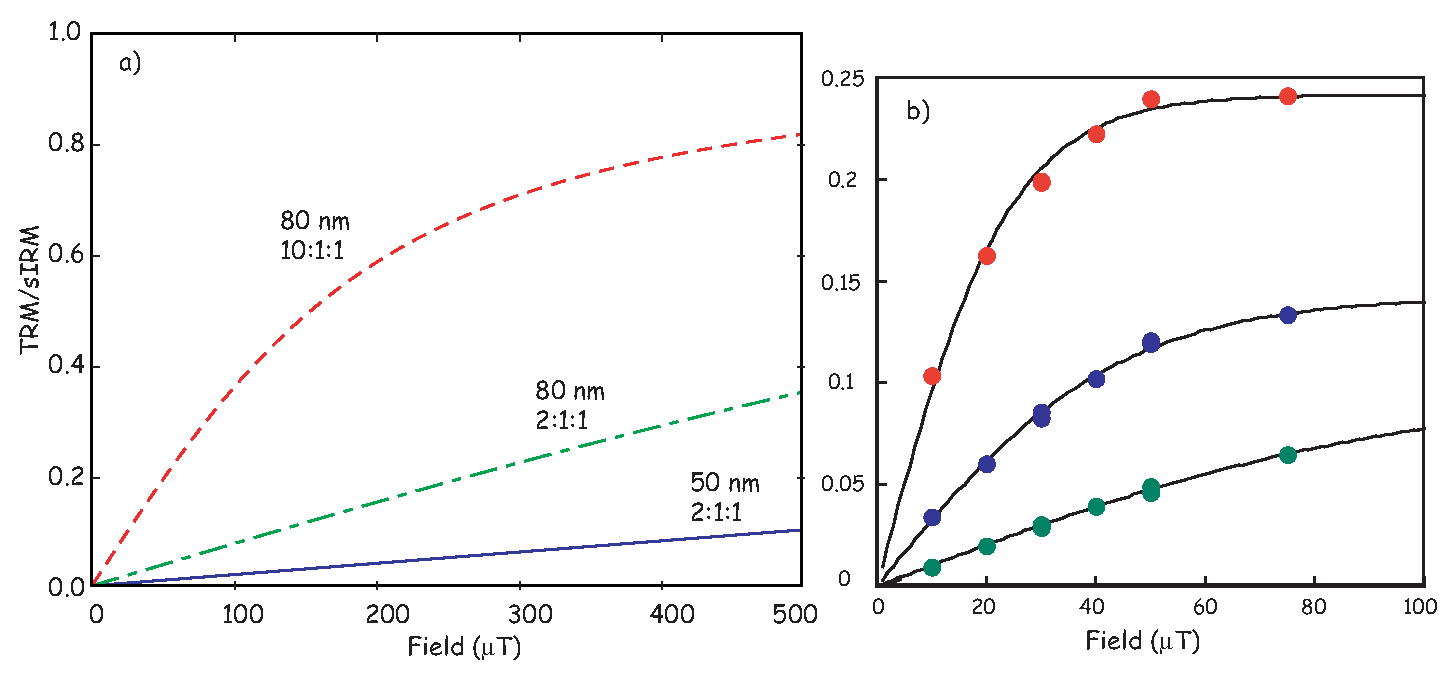
\includegraphics[width=14 cm]{EPSfiles/trm.eps}
\caption{Relationship of TRM with respect to the applied field for different assemblages of magnetite grains.  a) Theoretical calculations of TRM acquisition for different assemblages of randomly oriented non-interacting single domain ellipsoids of magnetite.  b) Experimentally determined TRM acquisition in three natural specimens. [Redrawn from Selkin et al., 2007.]}
\label{fig:trm}
\end{figure}  \nocite{selkin07}


We show the theoretical behavior of TRM as a function of applied field for different assemblages of particles in Figure~\ref{fig:trm}a.  This plot was constructed assuming ellipsoidal particles whose saturation magnetization varied according to Equation~\ref{eq:MsT} from Chapter 3 with $\gamma=0.38$.  For small, equant particles,  TRM is approximately linear with applied field for values of $B$ as small
as the Earth's ($\sim$ 20-65 $\mu$T).   However, the more elongate and the larger the particle, the more non-linear the theoretically predicted TRM behaves.  This non-linear behavior has been experimentally verified by 
\nocite{selkin07}
\index{Selkin, P.}
Selkin et al. (2007)  for geologically important materials (see Figure~\ref{fig:trm}b).  


\begin{figure}[htb]
%\epsfxsize 9cm
%\centering \epsffile{EPSfiles/pTRM.eps}
\centering  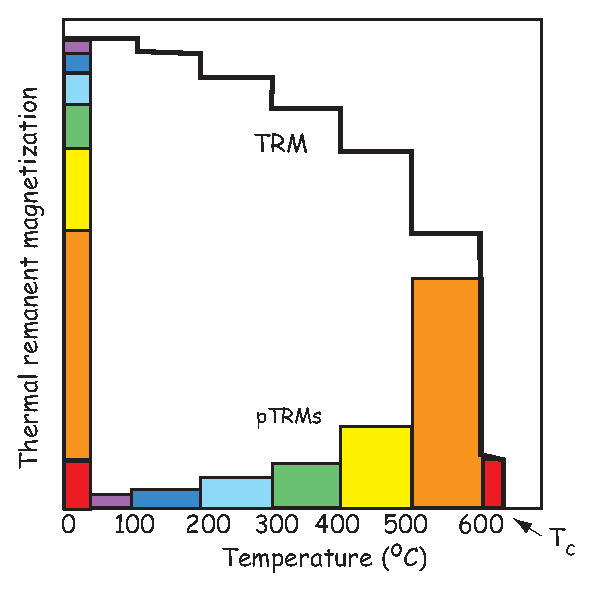
\includegraphics[width=9 cm]{EPSfiles/pTRM.eps}
\caption{Distribution of blocking temperatures
 of a typical basaltic specimen.
The solid line labeled TRM indicates
the amount of TRM remaining after
step heating to increasingly higher
temperature.   The colored blocks
 labeled PTRM
shows the amount of TRM blocked within
corresponding temperature intervals.  }
\label{fig:ptrm}
\end{figure}

The exact distribution of  blocking temperatures depends on the distribution of grain sizes and shapes in the rock and is
routinely determined in paleomagnetic studies.  By heating a rock in zero field to some temperature $T$,  grains with relaxation times that are superparamagnetic at that temperature become randomized, a process used in so-called 
\index{demagnetization!thermal}
{\it thermal demagnetization} which will be discussed further in Chapter 9.   Thermal demagnetization allows us to determine the portion of TRM that is blocked within successive blocking temperature intervals. A
typical example is shown in Figure~\ref{fig:ptrm}.   
The total TRM can be broken into portions acquired in distinct temperature intervals.   The portion of TRM
blocked in any particular blocking temperature window is referred to as
 \index{magnetization!remanent!thermal!partial}
{\it partial TRM},  often abbreviated pTRM. Each pTRM is a
vector quantity, and for single domain remanences,  the total TRM is the vector sum of the pTRMs contributed by all blocking temperature windows:
$$
\hbox{TRM}  = \sum_i^n \hbox{pTRM} (T_{bi}).
$$

According to
\index{N\'eel!theory}
 N\'eel theory for single domains, individual pTRMs depend only on the magnetic field during cooling through their respective blocking temperature  intervals and
are not affected by magnetic fields applied during cooling through lower temperature intervals. This is the
\index{Law of!additivity}
law of additivity of pTRM.  Another useful feature of pTRMs in single domain grains is that their blocking temperatures are the same as the temperature at which the remanence is unblocked, the so-called
\index{unblocking temperature}
 {\it unblocking temperature}  ($T_{ub}$).   This is the 
 \index{Law of!reciprocity}
 law of reciprocity.   While it may seem intuitively obvious that $T_b$ would be the same as $T_{ub}$, it is actually only true for single domain grains and fails spectacularly for multi-domain grains and even grains whose remanences are in the vortex state.  


As an example of the
\index{Law of!additivity}
 laws of additivity and reciprocity of pTRM, again consider our lava flow.  It originally cooled to produce a TRM that is the vector sum of all pTRMs with
$T_b$  distributed from $T_c$ to room temperature.  If the magnetic field was constant during the original cooling, all
pTRMs would be in the same direction. Now consider that this rock is subsequently reheated for even a short
time to a temperature, $T_r$,  intermediate between room temperature and the Curie temperature and then
cooled in a different magnetizing field. All pTRMs with $T_{ub} < T_r$ will record the new magnetic field direction.
However, neglecting time-temperature effects to be considered later, the pTRMs with $T_{ub} > T_r$ will retain the
TRM record of the original magnetizing field. This ability to strip away components of magnetization held by
grains with low unblocking temperatures while leaving the higher $T_{ub}$  grains unaffected is a fundamental element of the thermal
demagnetization technique to be discussed in later chapters.


\begin{figure}[htb]
%\epsfxsize 10cm
%\centering \epsffile{EPSfiles/trm-d.eps}
\centering  \includegraphics[width=10 cm]{EPSfiles/trm-d.eps}
\caption{Dependence of intensity of TRM on particle diameter of magnetite. Magnetite particles were
dispersed in a non-magnetic matrix; the intensity of TRM is determined per unit volume of magnetite and normalized to the maximum TRM observed to allow
comparison between experiments that used varying concentrations of dispersed magnetite; the
magnetizing field was 100 $\mu$T. [Data compiled by Dunlop and \"Ozdemir, 1997.]   }
\label{fig:trm-d}
\end{figure}\nocite{dunlop97}

Perhaps the most severe simplification in the above model of TRM acquisition is that it considers only
single-domain grains. Given the restricted range of grain size and shape distributions for stable SD grains
of magnetite or titanomagnetite (see Chapter 4), at most a small percentage of grains in a typical igneous rock are truly SD. The question then arises as to whether larger  grains can acquire TRM.

Figure~\ref{fig:trm-d}  shows the particle size dependence of TRM acquired by magnetite in a magnetizing field 100 $\mu$T.  Note that it is a log-log plot and efficiency of TRM acquisition very low
in the grain-size range from 1 $\mu$m to about 10 $\mu$m. However,  grains in 1-2 $\mu$m range do acquire TRM that can
be stable against time decay and against demagnetization by later magnetic fields.  This observation is the source of the term 
\index{pseudo-single domain}
 pseudo-single domain (PSD; see also Chapter 5) which characterizes the behavior of grains that are too large to be truly single domain, yet  do exhibit stability  unexpected for grains with domain walls (MD grains).  
The physics of PSD
grains is much more complicated than for SD grains and is not fully understood (see Section~\ref{sect:mixtures}  for a brief discussion.)
 
For grains larger than a few microns, the acquisition of TRM is very inefficient.  In addition, TRM in these larger
grains can be quite unstable; they are prone to acquire viscous magnetization.   SD and PSD grains are the effective carriers of TRM, while larger MD grains are likely
to carry a component of magnetization acquired long after original cooling.

Rapidly cooled volcanic rocks generally have grain-size distributions
with a major portion of the distribution within SD and PSD ranges. Also deuteric
oxidation of volcanic rocks can produce intergrowth grains with effective magnetic grain size less than the
magnetic grains that crystallized from the igneous melt. Thus, volcanic rocks are commonly observed to
possess fairly strong and stable TRM. A typical intensity of TRM in a basalt flow is 1 Am$^{-1}$. Because grain size depends in part on cooling rate of the igneous body,  rapidly cooled extrusive rocks are frequently preferable to slowly cooled intrusive rocks.   However, exsolution processes can break what would have been unsuitable MD magnetic grains into ideal strips of SD-like particles (see Chapter 6) so there is no universal rule as to which rocks will behave in the ideal single domain manner.     

\begin{figure}[htb]
%\epsfxsize 14cm
%\centering \epsffile{EPSfiles/neel-crm.eps}
\centering  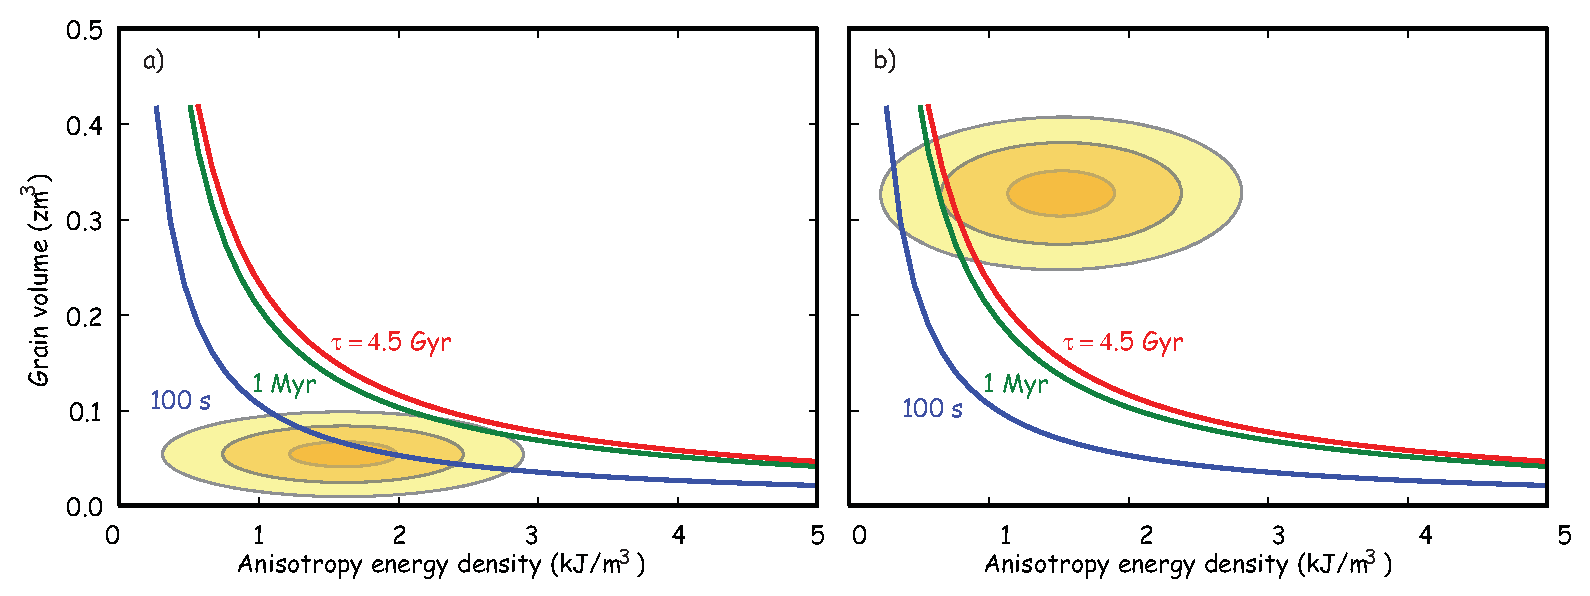
\includegraphics[width=14 cm]{EPSfiles/neel-crm.eps}
\caption{Migration of  the blocking energy of grains by increasing volume.  The relaxation times of a population of magnetic grains from a) short relaxation times when the particles are small  to b) long relaxation times when the grains have grown through their blocking volumes.    }
\label{fig:neel-crm}
\end{figure}


\section {Chemical remanent magnetization}
\label{sect:crm}

Equation~\ref{eq:tau3} shows that blocking energy depends on volume.  This means that relaxation time could change from very short to very long by increasing the size of the grain (see Figure~\ref{fig:neel-crm}).    
Chemical changes that form ferromagnetic minerals below their blocking temperatures which then grow  in a magnetizing field result in  acquisition of a {\it chemical remanent magnetization} or 
 \index{magnetization!remanent!chemical}
 Chemical reactions involving  ferromagnetic minerals include a) alteration of a pre-existing mineral (possibly also ferromagnetic) to a ferromagnetic mineral CRM. 
 \index{magnetization!remanent!chemical!alteration}
{\it alteration chemical remanence} aCRM or b) precipitation of a ferromagnetic mineral from solution.  This section outlines a model of CRM acquisition that explains the basic attributes of this type of
 \index{magnetization!remanent!chemical!grain-growth}
{\it grain-growth} CRM (gCRM).



\begin{figure}[htb]
%\epsfxsize 14cm
%\centering \epsffile{EPSfiles/crm.eps}
\centering  \includegraphics[width=14 cm]{EPSfiles/crm.eps}
\caption{Grain growth CRM. a) Red beds of the Chinji Formation, Siwaliks, Pakistan.  The red soil horizons have a CRM carried by pigmentary hematite.  b) Initial state of non-magnetic matrix.  c) Formation of superparamagnetic minerals with a statistical alignment with the ambient magnetic field (shown in blue). }
\label{fig:chinji}
\end{figure}

Magnetic mineralogy can change after a rock is formed in response to changing chemical environments.   Red beds (see Figure~\ref{fig:chinji}a), a dominant sedimentary facies in earlier times, are red because pigmentary hematite  grew at some point after deposition.  Hematite is a magnetic phase and the magnetic remanence it carries when grown at low temperatures is an example of gCRM.    

Magnetite is an example of a magnetic phase which is generally out of chemical equilibrium in many environments on the Earth's surface.  It tends to oxidize to another magnetic phase (maghemite) during weathering.  As it changes state, the iron oxide may change its magnetic moment, acquiring an 
 \index{magnetization!remanent!chemical!alteration}
aCRM.  

The relationship of the new born CRM to the ambient magnetic field can be complicated.  It may be largely controlled by the prior magnetic phase whence it came, it may be strongly influenced by the external magnetic field, or it may be some combination of these factors.  We will begin with the simplest form of CRM -- the gCRM.  

Inspection of Equation~\ref{eq:tau3}
 for relaxation time reveals that it is a strong function
of grain volume.  A similar theoretical framework can be built for remanence
acquired by grains growing in a magnetic field as for those cooling in a
magnetic field.   
As a starting point for our  treatment, consider a non-magnetic
porous matrix, say a sandstone.  As ground water percolates through the
sandstone, it begins to precipitate tiny grains of a magnetic mineral (Figure~\ref{fig:chinji}c). 
  Each crystal is completely isolated from its neighbors.  For very
small grains, the thermal energy dominates the system  and they are superparamagnetic. 
When  volume becomes sufficient for
magnetic anisotropy energy to overcome the 
thermal energy, the grain moment is
blocked and can remain out of equilibrium with the magnetic field 
for geologically
significant time periods.    Keeping temperature constant, there is
a critical 
\index{blocking!volume}
 {\it blocking volume} $v_b$ below which a grain maintains
equilibrium with the applied field and above which it does not.     We can find this blocking volume by solving for $v$ in the 
\index{N\'eel!equation}
N\'eel equation:   

\beq
v_b = { {kT\ln (C\tau)} \over {K_u} }.
\label{eq:vb}
\eeq


\noindent  The
magnetization acquired during grain growth is controlled by the alignment of
grain moments at the time that they grow through the blocking volume.      
Based on these principles, 
CRM should behave very similarly to TRM.

 There have been a few experiments carried out with an eye to testing
the grain growth CRM model  and although the theory predicts the zeroth order results quite well
(that a simple CRM parallels the field and is proportional to it in intensity), the
details are not well explained, primarily because the magnetic field affects the growth
of magnetic crystals and the results are not exactly analogous to TRM conditions
\index{Stokking, L.}
\index{Tauxe, L.}
(see e.g. Stokking and Tauxe, 1990a.)
\nocite{stokking90}
  Moreover, gCRMs acquired in  changing fields can be much more complicated than a simple single generation, single field gCRM (Stokking and Tauxe, 1990b). \nocite{stokking90b}    

Alteration CRM can also be much more complicated than simple gCRM in a single field.  Suffice it to say that the reliability of CRM for recording the external field must be verified (as with any magnetic remenance) with geological field tests  and other techniques as described in future chapters.  


\begin{figure}[h!tb]
%\epsfxsize 6.5cm
%\centering \epsffile{EPSfiles/lit-redep.eps}
\centering  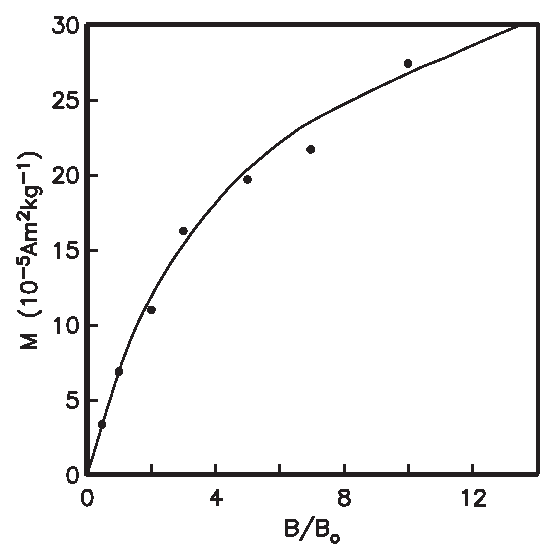
\includegraphics[width=6.5 cm]{EPSfiles/lit-redep.eps}
\caption{Depositional remanence versus applied field for redeposited glacial varves.  $B_o$ was the field in the lab.  [Data from Johnson et al., 1948; figure from Tauxe, 1993.]}
\label{fig:lit-redep}
\end{figure}
\nocite{johnson48,tauxe93}



\section {Detrital remanent magnetization}
\label{sect:drm}

Sediments become magnetized in quite a different
manner from igneous bodies.  Detrital grains are already magnetized, unlike
igneous rocks which crystallize above their 
Curie temperatures. Magnetic  particles that can rotate freely will turn into the direction of the applied field just as compass needles do.  The net magnetization of such particles, if locked in place can result in a 
 \index{magnetization!remanent!detrital}
{\it depositional remanent magnetization} (DRM).    Sediments are also subject to post-depositional modification through the action of organisms, compaction,  diagenesis  and the aquisition of VRM all of which will affect the magnetization.  This magnetization is usually called 
 \index{magnetization!remanent!post-depositional}
{\it post-depositional remanent magnetization} or pDRM.    In the following, we will consider the syn-depositional processes of physical alignment of magnetic particles in viscous fluids (giving rise to the primary DRM).


\subsection{Physical alignment of magnetic moments in viscous fluids}

 The theoretical  and experimental  foundation for DRM  is less complete than for TRM.     Placing a magnetic moment $\bf m$  in an applied field  $\bf B$ results in a torque  $\Gamma$ on the particle ${\bf \Gamma} = {\bf m} \times {\bf B} = mB\sin \theta$, where $\theta$ is the angle between the moment and the magnetic field vector.   In a fluid like water, the torque is opposed by the viscous drag and inertia so  the  equation of motion governing the approach to alignment  is: 
  
  \begin{equation}
 I  {{d^2 \theta}\over {dt^2}}  =- \lambda {{d \theta}\over {dt}} - m B \sin \theta, 
 \label{eq:motion}
\end{equation}
 
 \noindent where $\lambda$ is the viscosity coefficient opposing the motion of the particle through the fluid and $I$ is the moment of inertia.  Neglecting the inertial term (which is orders of magnitude less important that the other terms) we have:
 
 \begin{equation}
\tan {\theta \over 2} = \tan {\theta_o \over 2}{e}^{(-m B t/\lambda )},
\label{eq:nagata}
\end{equation}


\noindent where $\theta_o$ is the initial angle between ${\bf m}$ and ${\bf B}$ 
\nocite{nagata61} 
\index{Nagata, T.}
(Nagata, 1961).   By  setting  $\lambda=8\pi  r^3 \eta$ where $r$ is the particle radius and $\eta$ to the viscosity of water ($\sim  10^{-3}$ kg m$^{-1}$s$^{-1}$), the time constant $\Upsilon$ of Equation~\ref{eq:nagata} over which an inital $\theta_o$ reduces to $1/e$ of its value would be:
\begin{equation}
\Upsilon = {{\lambda}\over {mB}} = {  {6 \eta}\over {MB}},
\label{eq:Upsilon}
\end{equation}


\noindent where $M$ is the volume normalized magnetization. 


Plugging in reasonable values for $\eta, M$ and $B$ and assuming isolated magnetic particles yields a  time constant that  is extremely short (microseconds).    
The simple theory of unconstrained rotation of magnetic particles in water as developed by 
\nocite{nagata61}
\index{Nagata, T.}
Nagata (1961) predicts that sediments with isolated magnetic particles should have magnetic moments that are fully aligned and   insensitive to changes in magnetic field strength; DRM should be at saturation.    Yet even from the earliest days of laboratory redeposition experiments  (e.g., 
\nocite{johnson48}
\index{Johnson, E.A.}
Johnson et al., 1948; see Figure~\ref{fig:lit-redep}a) we have known that  depositional remanence (DRM) can have a strong field dependence and that DRMs are generally far less than saturation remanences  ($\sim$0.1\%).     Much of the research on DRM has focussed on explaining the strong  field dependence observed for laboratory redepositional DRM.    

\begin{figure}[htb]
%\epsfxsize 14cm
%\centering \epsffile{EPSfiles/drmprocesses.eps}
\centering  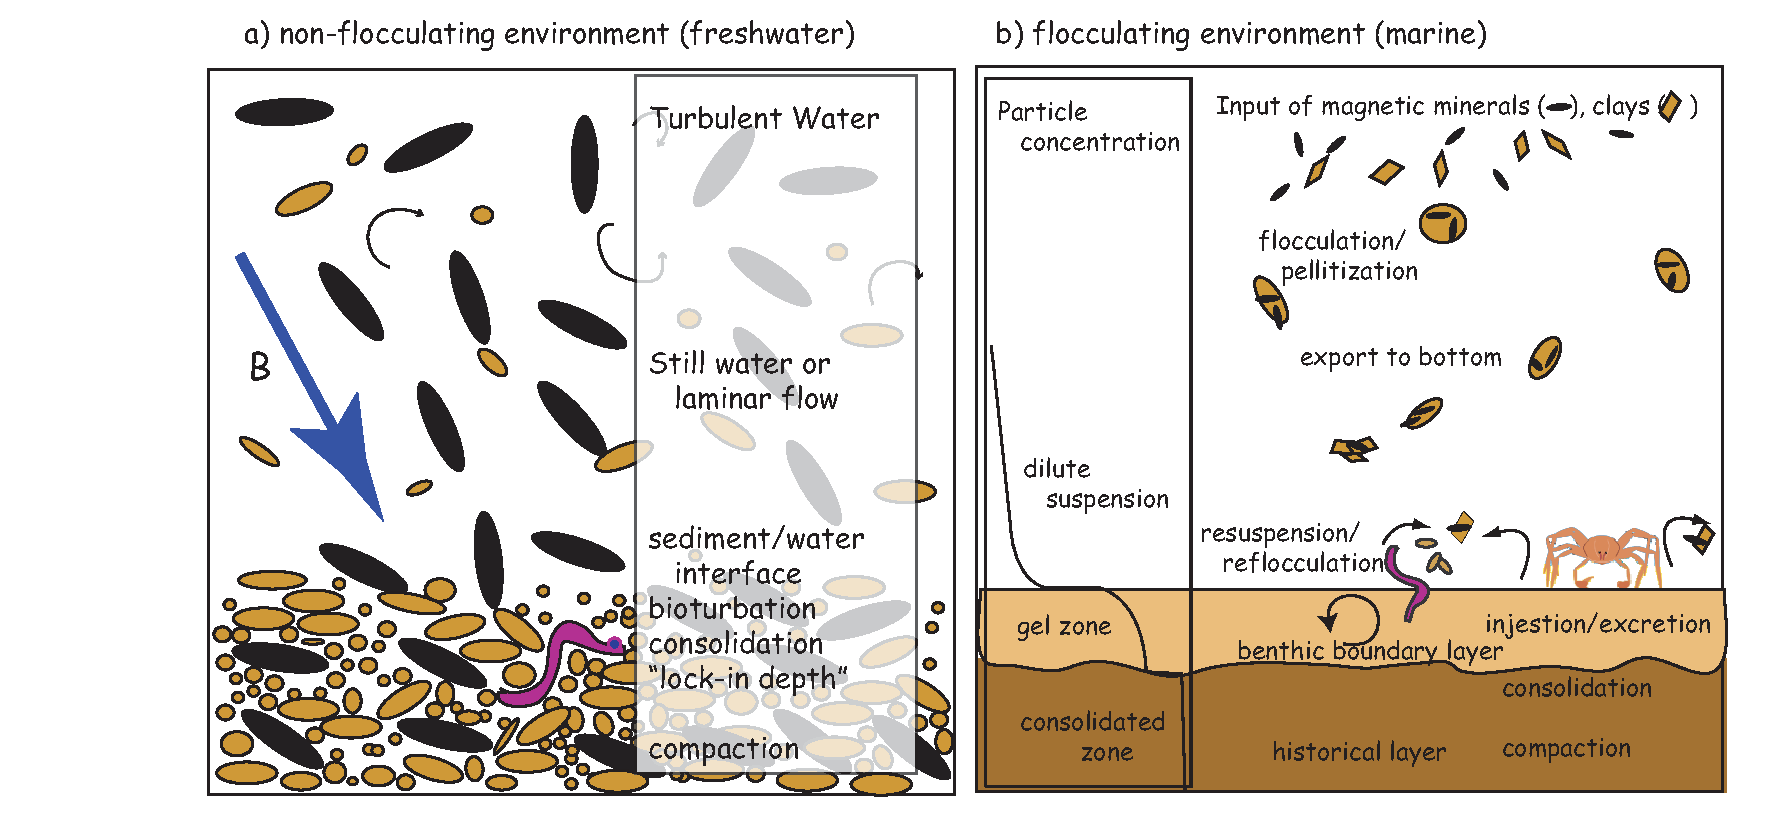
\includegraphics[width=14 cm]{EPSfiles/drmprocesses.eps}
\caption{a) Schematic drawing of traditional view of the journey of magnetic particles from the water column to burial in a non-flocculating (freshwater) environment. Magnetic particles are black.  b) View of depositional remanence in a flocculating (marine) environment.  [Figure from Tauxe and Yamazaki, 2007.] }
\label{fig:drmprocesses}
\end{figure}\nocite{tauxe07}



The observation that DRM is usually orders of magnitude less than saturation and that it appears to be sensitive to changing geomagnetic field strengths implies that the time constant of alignment is much longer than predicted by Equation~\ref{eq:Upsilon}.   Either there is a disruption of alignment by some mechanism, or we have underestimated $\Upsilon$ somehow.  

Collinson (1965) \nocite{collinson65} invoked Brownian motion to disrupt alignment.  Reasonable parameter assumptions suggest that particles smaller than about 100 nm could be affected by Brownian motion suggesting a possible role in DRM of isolated magnetite grains free to rotate in water.   The problem with this suggestion is that such small particles take an extremely long time to settle.  Also, in almost all natural waters, magnetite particles will adhere to clay particles making isolated magnetic particles  in nature unlikely (see, e.g., Katari et al., 2000). \nocite{katari00}     

To increase $\Upsilon$, one can either assume a larger viscosity than that of pure water, or decrease magnetization. by for example, using values   for $M$ much lower than the saturation magnetizations of common magnetic minerals (e.g.,  \nocite{collinson65}
\index{Collinson, D.W.}
Collinson, 1965) or padding the magnetic particles with non-magnetic ``fluff'' through the process of flocculation 
\index{Shcherbakov, V.P.}
\index{Shcherbakova, V.V.}
(Shcherbakov and Shcherbakova, 1983).    \nocite{shcherbakov83}
Using the viscosity in the sediment itself  in Equation~\ref{eq:Upsilon} fails to explain laboratory remanences that are demonstrably ``fixed'' after settling -- the viscosity of the mud appears to be too high to allow post-depositional  re-alignment, yet these sediments exhibit field dependence (e.g., Tauxe et al., 2006).   \nocite{tauxe06}
Alternatively, one could increase  $\Upsilon$ by  assuming a reduce value for $M$.  However, even using the magnetization of hematite, which is two orders of magnitude lower than magnetite, results in values for $\Upsilon$ that are still less than a second.  

  In  saline environments, sedimentary particles tend to flocculate.    For magnetic particles embedded in a non-magnetic matrix,   the magnetic field must turn the entire particle and the net magnetization of the floc  must be used in Equation~\ref{eq:Upsilon}.    



\begin{figure}[htb]
%\epsfxsize 14cm
%\centering \epsffile{EPSfiles/brownian.eps}
\centering  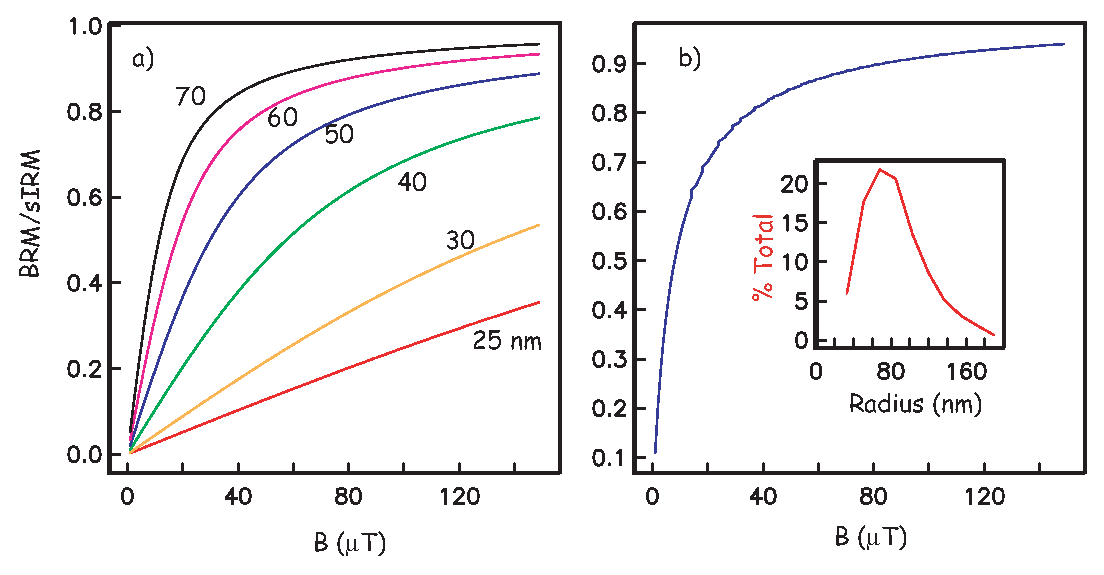
\includegraphics[width=14 cm]{EPSfiles/brownian.eps}
\caption{a) Numerical simulations of Brownian remanent magnetization (BRM) for various sizes of magnetite.  b) BRM simulated for distribution of particle sizes of magnetite shown in inset.  [Figure from Tauxe and Yamazaki, 2007.]}
\label{fig:brownian}
\end{figure}

 The tendency to flocculate 
 increases with increasing salinity. 
There are therefore  two completely different systems when discussing DRM: ones in which magnetic particles remain essentially isolated  or embedded in very small flocs (e.g., in freshwater lakes; see Figure~\ref{fig:drmprocesses}a) and 
ones in which flocculation plays a role (e.g., marine environments; see Figure~\ref{fig:drmprocesses}b).   
For the case of magnetite in freshwater, Brownian motion may reduce DRM efficiency and give rise to the dependence on $B$.   In saline waters,  however, the most important control on DRM  is the size of the flocs in which the magnetic particles are embedded.      In the following we briefly explore these two very different environments.


\subsubsection{Non-flocculating environments}

In freshwater we expect to have relatively unflocculated particles whose magnetic moments are presumably a saturation remanence.    Although, even in fresh water, the magnetic particles are likely to be attached to clays through van der Waals attraction  the clays themselves have no great mutual attraction.    It is possible, therefore that magnetic particles could be subject to Brownian motion.   Here we outline the theory to investigate the behavior of DRM that would be expected from a Brownian motion mechanism (henceforth a
 \index{magnetization!remanent!Brownian}
{\it  Brownian remanent magnetization}  or BRM).   

To estimate the size of particles affected by Brownian motion, 
\nocite{collinson65}
\index{Collinson, D.W.}
Collinson  (1965) used the equation:

\begin{equation}
{1\over 2} mB\phi^2 = {1\over 2} kT,
\label{eq:collinson}
\end{equation}

\noindent where $\phi$ is the Brownian deflection about the applied field direction (in radians), $k$ is Boltzmann's constant (1.38 x 10$^{-23}$JK$^{-1}$) and $T$ is the temperature in kelvin.    The effect of viscous drag on particles may also be important  when the magnetic moments of the particles are low  (see 
 \nocite{coffey96}
\index{Coffey, W.T.}
 Coffey et al., 1996 for a complete derivation), for which we have:

$$
{ {\phi^2}\over{\delta}}= {{kT}\over {4\pi \eta r^3}},
$$

\noindent where $\delta$ is the time span of observation (say, 1 second).  According to this relationship, weakly magnetized particles smaller than about a micron will  be strongly affected by Brownian motion.   Particles that have a substantial magnetic moment however, will be partially stabilized (according to Equation~\ref{eq:collinson}) and might remain unaffected by Brownian motion to smaller particle sizes (e.g., 0.1 $\mu$m).    In the case of isolated particles of magnetite, therefore, we should use Equation~\ref{eq:collinson} and BRM should follow the Langevin equation   for paramagnetic gases, i.e.:  

\begin{equation}
{ BRM\over{sIRM} } = { \hbox{coth} \bigl( {mB \over {kT}}\bigr)  - { kT \over {mB} }}.
\label{eq:brm}
\end{equation}

\noindent Here the quantity sIRM is a saturation isothermal remanence ($M_r$ in Chapter 5) and is the moment acquired when all the magnetic particles are aligned to the maximum extent possible.  To get an idea of how BRMs would behave, we first find $m$ from $M(r)$ [here we use the results from micromagnetic modeling (see Chapter 4)].     Then, we  evaluate Equation~\ref{eq:brm} as a function of $B$ for a given  particle size (see Figure~\ref{fig:brownian}a).     We can also assume any  distribution of particle sizes (e.g, that shown as the inset to Figure~\ref{fig:brownian}b), and  predict BRM/sIRM for the distribution (blue line in Figure~\ref{fig:brownian}b).   It is interesting to note that BRMs  are almost never linear with the applied field unless the particle sizes are very small.    




BRMs are   fixed when the particles are no longer free to move.  The fixing of this magnetization presumably occurs during consolidation, at a depth (known as the lock-in depth) where the porosity of the sediment reduces to the point that the particles are pinned (see Figure~\ref{fig:drmprocesses}a).  Below that, the magnetization may be further affected by 
\index{compaction}
compaction (e.g., 
\nocite{deamer90}
\index{Deamer, G.A.}
\index{Kodama, K.P.}
Deamer and Kodama, 1990)  and diagenesis (e.g., 
\nocite{roberts95}
\index{Roberts, A.P.}
Roberts, 1995).


\begin{figure}[htb]
%\epsfxsize 13cm
%\centering \epsffile{EPSfiles/flocs.eps}
\centering  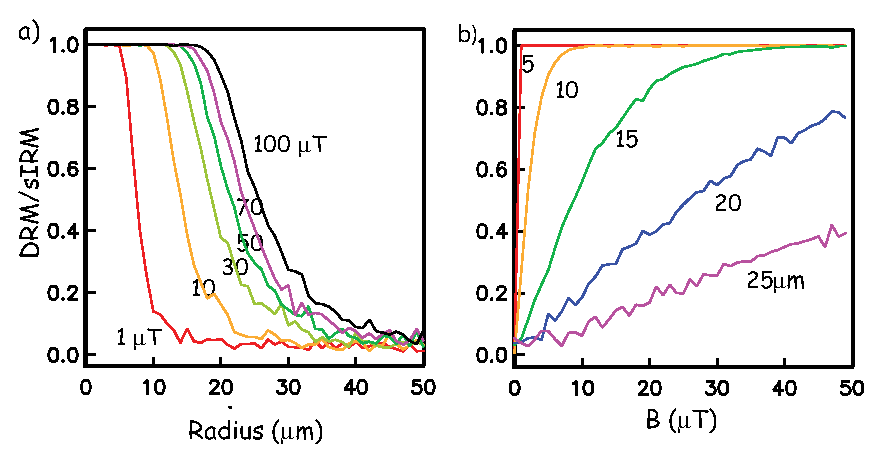
\includegraphics[width=13 cm]{EPSfiles/flocs.eps}
\caption{a)  Results of numerical experiments of the flocculation model using the parameters: $l=0.2$ m and the viscosity of water.  $M/M_o$ is the DRM expressed as a fraction of saturation, holding $\bar m$ constant and varying $B$.  For a given field strength, particles are either at saturation or randomly oriented, except for within a very narrow size range.  b) Same as a) but plotted versus applied field ($B$). [Figures  from Tauxe et al., 2006.]   }
\label{fig:flocs}
\end{figure}\nocite{tauxe06}
\subsubsection{Flocculating environments}
\label{sect:flocs}


  Equation~\ref{eq:nagata} predicts that a  magnetic moment $\bf m$ making an initial angle $\theta_o$ with the applied field  $\bf B$  will make an angle $\theta$ with the field after time $t$.  From this, we can make a simple numerical model to predict the DRM for an initially randomly oriented assemblage of magnetic moments, after time $t$ [or the equivalent settling length $l$ using some settling law (e.g.,
   \nocite{gibbs85} 
   \index{Gibbs,  R.}
   Gibbs  1985; see \nocite{katari01}
   \index{Katari, K.}
   \index{Bloxham, J.}
   Katari and Bloxham 2001)].  In Figure~\ref{fig:flocs}a and b, we show the DRM curves predicted by 
   \nocite{tauxe06}
   \index{Tauxe, L.}
   Tauxe et al. (2006) for simple flocs with a single magnetite grain in each  as a function of magnetic field and radius. 
  
   In general, the magnetic flocs are either nearly aligned with the magnetic field, or nearly random with only a narrow band of floc sizes in between the two states for a given value of $B$.  Increasing $B$ increases the size for which particles can rotate into the field, giving rise to the dependence of DRM intensity on applied field strength.   Taking a given particle size and evaluating DRM as a function of the applied field (Figure~\ref{fig:flocs}b)  predicts  the opposite behavior for DRM than the Brownian motion approach (Figure~\ref{fig:brownian}) in that the larger the floc size, the weaker the DRM and also the more linear with respect to the applied field.     Brownian motion, therefore, predicts low DRM efficiency for the smallest particles  increasing to near saturation values for particles around 0.1 $\mu$m while composite floc theory  predicts decreased  DRM efficiency for larger floc sizes.   

\begin{figure}[htb]
%\epsfxsize 8cm
%\centering \epsffile{EPSfiles/drm-exp.eps}
\centering  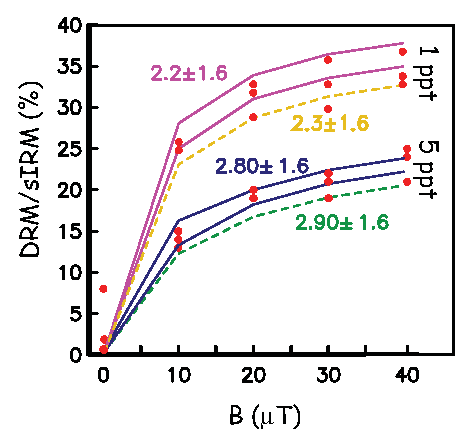
\includegraphics[width=8 cm]{EPSfiles/drm-exp.eps}
\caption{
Results of settling  experiments as a function of field ($B$) in a flocculating environment.    The assumed mean and standard deviations of truncated log-normal distributions for floc radii are shown in the legends  and are indicated using the different line styles in the figure.    [Figure from  Tauxe and Yamazaki, 2007 after Tauxe et al. 2006.]}
\label{fig:drm-exp}
\end{figure}

The flocculation model of DRM  makes specific predictions which can in principle be tested if the model parameters can be estimated or controlled.  Tauxe et al. (2006)  tested the flocculation hypothesis by dispersing  natural sediments in settling tubes to which varying amounts of NaCl had been introduced.   Prior to dispersal, each specimen of mud was given a saturation remanence.  They measured DRM as a function of salinity (and therefore floc size) and the applied field (see Figure~\ref{fig:drm-exp}).    In general their results suggested the following:
1)  the higher the salinity,  the lower the net moment and the   faster the particles settled,  2) the higher the applied field, the  higher the net moment, although a saturation DRM appeared to be nearly achieved in the 1 ppt NaCl set of tubes by 30 $\mu$T (Figure~\ref{fig:drm-exp}),  3)  the relationship of DRM to $B$ was far from linear with applied field in all cases, and 4) the saturation DRM was less than the saturation IRM so the simplest idea of one floc/one magnetic particle failed to explain the data.  

 In nature, flocs are formed by coalescing of ``fundamental flocs'' into composite flocs.  Each fundamental floc would have tiny magnetic particles adhering to them and would have the sIRM imparted prior to settling.  As the composite flocs grow by chance encounters with other flocs, the net moment of the composite floc will be the vector sum of the moments of the fundamental flocs.  Tauxe et al. (2006) used the composite floc hypothesis to  model  experimental DRMs (see examples in Figure~\ref{fig:drm-exp}); model predictions were  in excellent agreement with the redeposition data.  


\begin{figure}[htb]
%\epsfxsize 7cm
%\centering \epsffile{EPSfiles/ifio.eps}
\centering  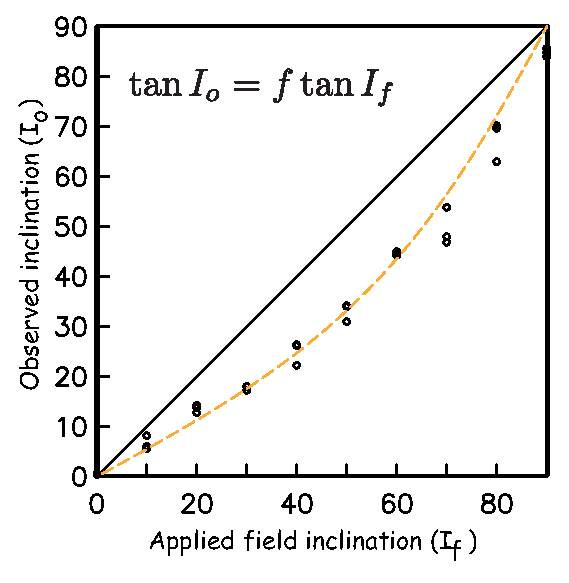
\includegraphics[width=7 cm]{EPSfiles/ifio.eps}
\caption{Applied field inclination versus remanent inclination for redeposited river sediments.  Best fit line is with $f=0.55$.   [Data from Tauxe and Kent, 1984.]   }
\label{fig:incerror}
\end{figure}
\nocite{tauxe84}



\subsection{Post-depositional processes}

It appears that by combining the effects of Brownian motion for non-flocculating environments and a composite floc model for flocculating environments  we are on the verge of a quantitative physical theory that can account for the acquisition of depositional remanence near the sediment/water interface.  The DRM will be fixed when no further physical rotation of the magnetic particles in response to the geomagnetic field is possible.  The depth at which moments are pinned is called the lock-in depth.    In the ``standard model'' of depositional  remanence (DRM) acquisition (see, e.g., 
 \nocite{verosub77} 
 \index{Verosub, K.}
 Verosub, 1977) detrital remanence is acquired by locking in different grains over a range of depths.  This phased lock-in  leads to  both  significant smoothing and to an offset between the sediment/water interface and the fixing of the DRM.   Many practitioners of paleomagnetism still adhere to this concept of DRM which stems from the early laboratory redeposition experiments which were carried out under non-flocculating conditions, however.    As summarized by 
 \nocite{tauxe06}
 \index{Tauxe, L.}
 Tauxe et al. (2006), the evidence for substantial smoothing and a deep ($>$10 cm)  lock in remains weak.  



Physical rotation of particles in response to compaction can also change the magnetic remanence.    
As sediments lose water and consolidate, compaction can have a strong effect on DRM intensity (e.g., \nocite{anson87} 
\index{Anson, G.L.}
\index{Kodama, K.P.}
Anson and Kodama, 1987).    Consolidation is a continuous process starting from the sediment water interface when sedimentary particles first gel (see, e.g., Figure~\ref{fig:drmprocesses}b) and continuing until the sediment is completely compacted, perhaps as deep as hundreds of meters.     The effect on magnetic remanence depends on volume loss during compaction which depends largely on clay content, so clay rich sediments will have the largest effect.     

Other processes not involving post-depositional physical rotation of magnetic particles including ``viscous'' (in the sense of magnetic viscosity) remagnetization and diagenetic alteration resulting in a chemical remanence may also modify the DRM.  All of these processes influence the  intensity of remanence and hamper our efforts to decipher  the original geomagnetic  signal.    


 
\subsection{Inclination Error}

Some sedimentary remanences  show a remanence vector that is
generally shallower than the applied field,
 a phenomenon known as
 \index{inclination!error}
{\it inclination error}.  We show the results of a typical laboratory redeposition experiment 
\index{Tauxe, L.}
\index{Kent, D.V.}
(Tauxe and Kent, 1984) \nocite{tauxe84}  in Figure~\ref{fig:incerror}.  The tangent of the observed inclination is usually
some fraction ($\sim$ 0.4-0.6) of the tangent of the applied field 
\index{King, R.F.}
(King 1955).   \nocite{king55} 
 Thus, inclination error is at a
maximum at 45$^{\circ}$ and is negligible at high and low inclinations.   Tauxe and Kent (1984) also demonstrated a strong link between DRM efficiency and inclination error.  Sediments exhibiting inclination error have the strongest remanences in horizontal fields and the weakest in vertical fields.   

Interestingly,  many natural sediments (e.g.
 deep sea or slowly deposited lake sediments) display no
inclination error.   The worst culprits appear to be sediments whose NRM is carried by detrital hematite, a flakey particle with a small saturation remanence.  


 \begin{figure}[htb]
 %\epsfxsize 14cm
 %\centering \epsffile{EPSfiles/lightning.eps}
 \centering  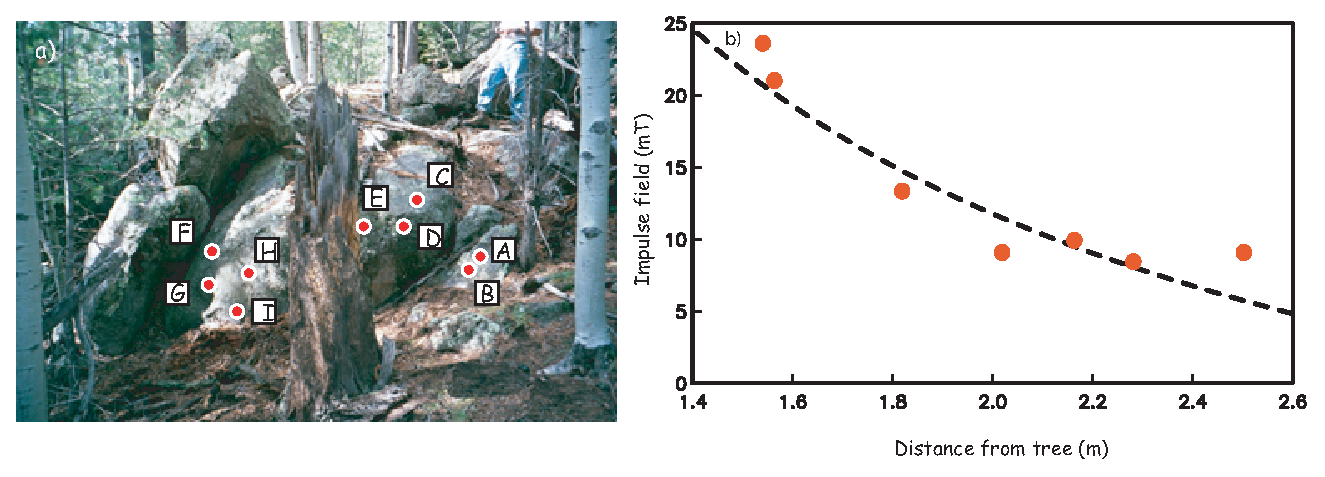
\includegraphics[width=14 cm]{EPSfiles/lightning.eps}
 \caption{Outcrop photo showing sampling locations and charred stump of tree that was hit by lightning in foreground.  b) Impulse field required to reproduce the NRM intensity as an IRM, plotted as a function of distance from the tree shown in
a). Dashed line is best-fit to the data assuming that the tree at the center of the photo was the site of a remagnetizing
line current (lightning bolt) of 300,000 Amps. [Figures from Tauxe et al., 2003.]}
 \label{fig:lightning}
 \end{figure} \nocite{tauxe03b}

 
\section {Isothermal remanent magnetization}
\label{sect:irm}

 Examination of the Equations~\ref{eq:tau2} and ~\ref{eq:tau3}  reveals an interesting dependence of relaxation time on the coercivity  of magnetic particles.  We can coax the magnetization of otherwise  firmly entrenched particles to follow an applied field, if that field is larger than the coercivity.  Exposing a particle to a large magnetic field, will allow magnetic particles whose coercivity is below that field to flip their magnetic moments to a direction at a more favorable angle to the applied field, resulting in a gain in magnetic remanence in that direction. This type of magnetic remanence is called an
 \index{magnetization!remanent!isothermal}
  {\it isothermal remanent magnetization} or IRM (see Chapters 4 and 5). 
  
 IRM is unfortunately a naturally occurring remanence.  When 
 lightning strikes in the neighborhood,  rocks can  become either partially or entirely remagnetized (see Figure~\ref{fig:lightning}).    These magnetizations often mask the primary magnetization (TRM or DRM), but can sometimes be removed.   
 
 IRMs can also be useful.  The magnitude is sensitive to the magnetic mineralogy, concentration and grain size and properties of IRMs are used for a variety of purposes, some of which we will discuss in Chapters 8 and 10.  
In anticipation of those chapters, we will briefly introduce some of properties of laboratory acquired IRMs.


\begin{figure}[htb]
%\centering \epsffile{EPSfiles/irm.eps}
\centering  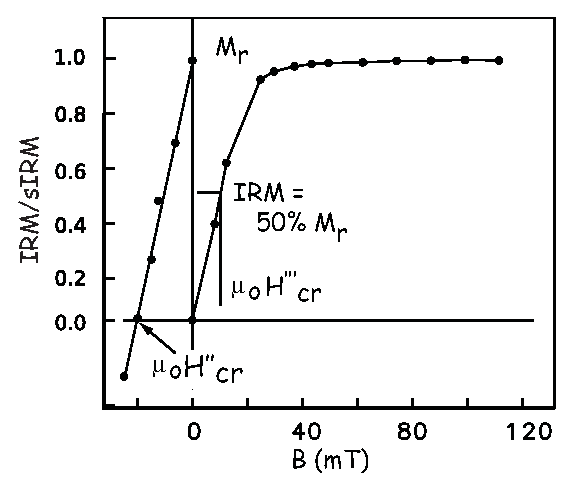
\includegraphics{EPSfiles/irm.eps}
\caption{Acquisition of IRM by exposure to large magnetic fields.  After saturation, the remanence remaining is $M_r$.  One can then turn the sample around and applied smaller fields in the opposite direction to determine the field necessary to reduce the net remanence to zero.   Also shown are two methods of estimating coercivity of remanence ($H_{cr}''$ and $H_{cr}'''$; see Appendix C for summary).
 }
\label{fig:irm}
\end{figure}


 In Figure~\ref{fig:irm} we illustrate the behavior of an initially demagnetized specimen as it is subjected to increasing impulse fields.  The maximum IRM achieved is known as 
 \index{magnetization!remanent!isothermal!saturation}
 sIRM (saturation IRM) or $M_r$ (and sometimes $M_{rs}$).  After saturation, the specimen can be turned around and subjected to increasingly large  
\index{coercivity!of remanence!estimation!back-field method}
 {\it back-fields}.  The back-field field sufficient to remagnetize half of the moments (resulting in a net remanence of zero) is the coercivity of remanence ($H_{cr}$ or $\mu_o H_{cr}$ depending on the magnetic units).    Alternatively, we  could use the magnetic field required to impart an IRM that is half the intensity of the saturation remanence ($H'''_{cr}$).   We call this the $H_{1/2}$ method.  
 
 
  
  

  
  By now we have encountered four different methods for estimating the coercivity of remanence (see Table~\ref{tab:hystpars}).  Each of these requires a monogenetic populations of grains and will give meaningless numbers if there are several different minerals or grain size populations in the specimen.  The ``ascending loop intercept method'' also assumes uniaxial single domain particles.  So differences between, for example the $H_{cr}$ estimate and $H_{cr}'$ could provide clues about departures from that  assumption.    
  


\section{Thermo-viscous remanent magnetization}

Sometimes rocks are exposed to elevated temperatures for long periods of 
time (for example during deep burial). The grains with relaxation times
(at the elevated temperature) shorter than the exposure time may have
acquired a so-called 
 \index{magnetization!remanent!thermo-viscous}
{\it thermo-viscous remanent magnetization} (TVRM).  To erase this remanence, the rock must be heated in the laboratory (in zero field) hot enough and long enough.  We cannot wait for geologically meaningful periods of time, so we must estimate what the effective blocking temperature of the TVRM component will be on laboratory time scales.   To do this,  we follow the logic of 
\index{Pullaiah, G.}
 Pullaiah et al. (1975).    \nocite{pullaiah75} If we hold $H_c, M_s$ and $v$ constant in Equation~\ref{eq:tau3}, we could calculate the
relationship of $\tau$ to temperature by:


$$
T_1 \ln C \tau_1 = T_2 \ln C \tau_2.
$$
But
$H_c$  and $M_s$  are also functions of temperature and  a more appropriate equation would be:
\beq
{{T_1 \ln C \tau_1} \over {M_s(T_1) H_c (T_1)}} = {{ T_2 \ln C \tau_2}
\over {M_s(T_2) H_c (T_2)}}.
\label{eq:pullaiah1}
\eeq


\noindent
For uniaxial anisotropy,  $H_c(T)\simeq \Delta N M_s$ for magnetite,  so  $H_c$ varies linearly with $M_s$.  
Exploiting this property, we can simplify Equation~\ref{eq:pullaiah1} to:

\beq
{{T_1 \ln C \tau_1} \over {M_s^2(T_1) }} = {{ T_2 \ln C \tau_2}
\over {M_s^2(T_2) }}.
\label{eq:pullaiahM}
\eeq


Now all we need is the variation of saturation magnetiztation with temperature.  As previously noted, this is not perfectly known.  However, using the approximate relationship from Chapter 3 of $M_s(T)$ ($\gamma$=0.38  in Equation ~\ref{eq:MsT} and assuming $T_c=580^{\circ}$C  as in Chapter 6), we  can draw the plot shown in Figure~\ref{fig:pullaiah}a   for
$\tau$ versus  $T_b$.   This plot is different in detail from that of 
\index{Pullaiah, G.}
\nocite{pullaiah75}
Pullaiah et al. (1975) because of the difference in assumed $M_s(T)$ behavior.  

The theoretical treatment for hematite is different than for magnetite because the dominant source of anisotropy is either a defect moment or magnetocrystalline anisotropy, and the relationship of coercivity with temperture is different than for shape anisotropy.  In fact, this relationship for hematite is very poorly constrained.  \index{Pullaiah, G.}
Pullaiah et al. (1975) assumed  $H_c(T)\propto M_s^3(T) $ from which they derived:

\beq
{{T_1 \ln C \tau_1} \over {M_s^4(T_1) }} = {{ T_2 \ln C \tau_2}
\over {M_s^4(T_2) }}.
\label{eq:pullaiahH}
\eeq

\noindent Using experimental values of blocking temperature for hematite, they calculated  nomograms for hematite similar to that shown in Figure~\ref{fig:pullaiah}b.   


\begin{figure}[htb]
%\epsfxsize 14cm
%\centering \epsffile{EPSfiles/pullaiah.eps}
\centering  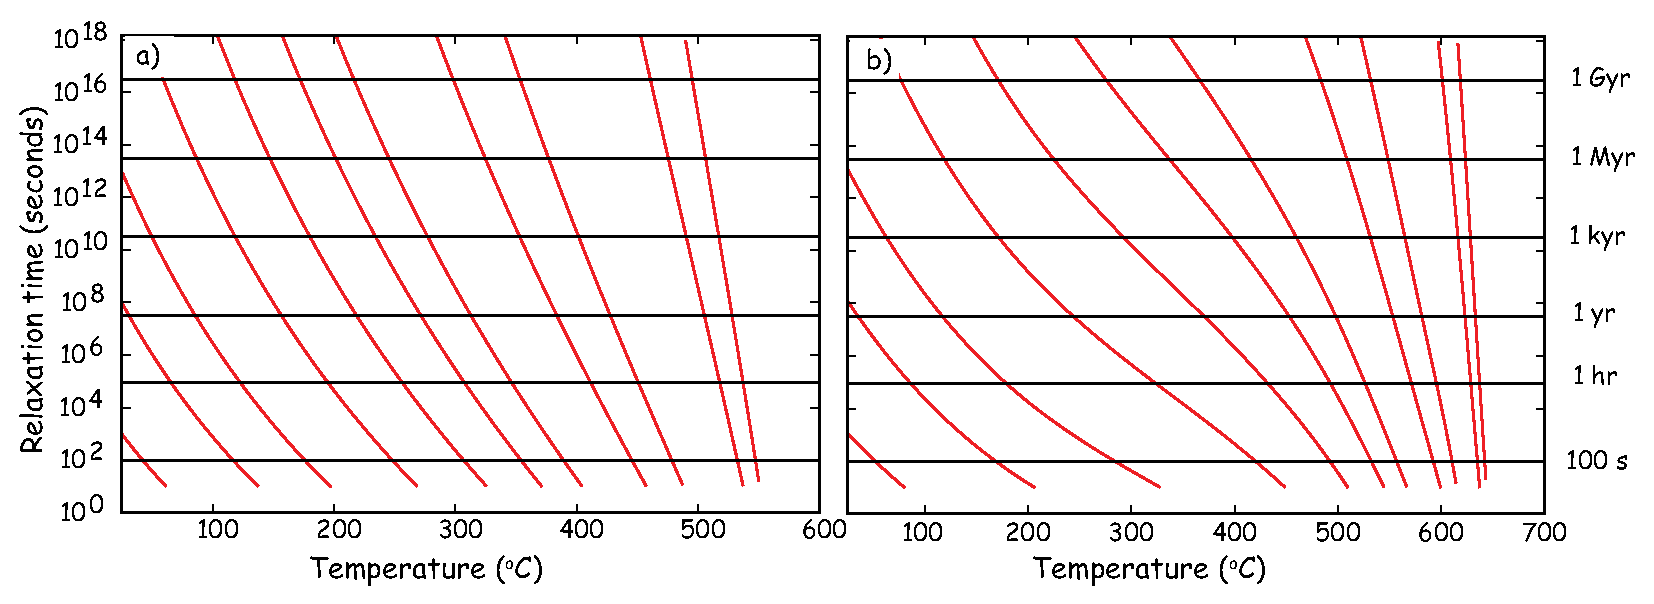
\includegraphics[width=14 cm]{EPSfiles/pullaiah.eps}
\caption{Theoretical nomogram relating relaxation time and blocking temperature.  a)   magnetite and b) hematite. }
\label{fig:pullaiah}
\end{figure}




Curves like those shown in Figure~\ref{fig:pullaiah} allow us to predict what the blocking temperature of a viscous magnetization acquired over many years will be under laboratory conditions (relaxation times of hundreds of seconds).   There are many assumptions built into the plot shown in Figure~\ref{fig:pullaiah} and some discussion in the literature (see 
\index{Dunlop, D.J.}
\index{\"Ozdemir, \"O.}
Dunlop and \"Ozdemir, 1997 \nocite{dunlop97} for a good summary).    Because of the sensitivity to the $M_s(T)$ behavior and the even more poorly constrained (at least for hematite) $H_c(T)$ behavior, these plots should be used with caution.    





\section {Natural remanent magnetization}

A rock collected from a geological formation has a magnetic remanence which may have been
acquired by a variety of mechanisms some of which we have described.  The remanence of
this rock is called 
simply a 
 \index{magnetization!remanent!natural}
 natural remanent magnetization  in order to avoid a
genetic connotation in the absence of other compelling evidence.  The NRM is often a
combination of several components, each with its own history.  The NRM must be picked
apart and the various components carefully 
analyzed before origin can be ascribed. The procedures for doing this
are described in later chapters.  


\begin{figure}[htb]
%\epsfxsize 9cm
%\centering \epsffile{EPSfiles/ARM.eps}
\centering  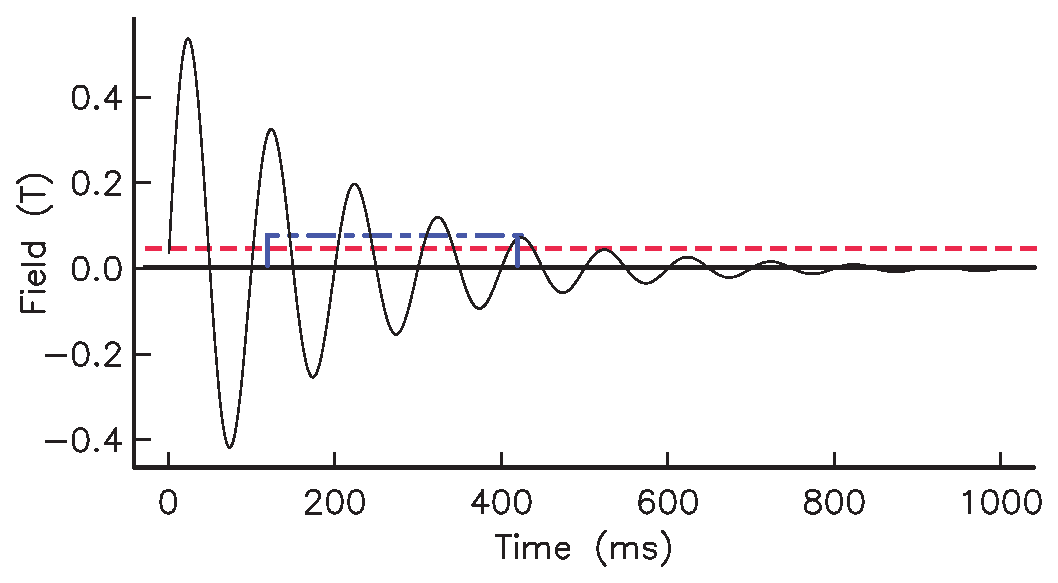
\includegraphics[width=9 cm]{EPSfiles/ARM.eps}
\caption{Acquisition of ARM in alternating magnetic field.  A total ARM is acquired if the DC field is switched on throughout the experiment (red dashed  line)  and a partial ARM (pARM) is acquired if the field is switched on only for part of the experiment (blue dash-dot line).  }
\label{fig:arm}
\end{figure}


\section{Artificial remanences }
\label{sect:arm}

Another way to magnetize rocks (although not in nature) is to subject a sample to 
an alternating field  (see Figure~\ref{fig:arm}).   Particles whose coercivity is lower than the peak oscillating field will flip and flop along with the field.   These entrained moments
will become stuck as the peak field gradually decays below the
coercivities of individual grains.   Assuming that there is a range of
coercivities in the sample, the low stability grains will be stuck half along
one direction of the alternating field and half along the other direction; the net
contribution to the remanence will be zero.  This is the principle of so-called
\index{demagnetization!alternating field}
 {\it alternating field (AF) demagnetization} which we will discuss in later chapters.   

If there is a small DC bias field superposed on the alternating field, then there will be a statistical
preference in the remagnetized grains for the direction of the bias field,   analogous to
TRM acquired during cooling.  This net magnetization is termed the {\it anhysteretic remanent magnetization} or ARM. 
\index{magnetization!remanent!anhysteretic}
 By analogy to partial thermal remanence, one can impart a partial anhysteretic remanence (pARM) by only turning on the DC field for part of the AF cycle (solid blue line in Figure~\ref{fig:arm}).    Also, by normalizing the magnetization (volume normalized with units of Am$^{-1}$) by the DC field (also converted to Am$^{-1}$), one has the dimensionless parameter known as ARM susceptibility ($\chi_{ARM}$).   This parameter assumes that ARM is linearly related to the inducing field so that $\chi_{ARM}$ is independent of the applied field.  This is of course only true for small DC fields and may not be true for the fields used in most laboratories (50-100 $\mu$T).    


A related remanence known as the
 \index{magnetization!remanent!gyro-}%
 {\it gyromagnetic remanent magnetization} or  GRM is a somewhat mysterious remanence that is acquired by stationary specimens in moving fields or by rotating specimens in either steady or moving fields.    It is most frequently observed as a component of magnetization acquired during alternating field demagnetization that is perpendicular to the last axis of demagnetization.   
  It was originally thought to arise from the gyroscopic response of SD moments to the torque of an applied field which, in anisotropic distributions of SD moments resulted in a net moment perpendicular to the applied field
   \index{Stephenson, A.}
 (Stephenson, 1981). \nocite{stephenson81}  But, truly uniaxial single domain particles will have no net remanence if demagnetized along all three axes, no matter how anisotropic the distribution of easy axes is.  More recently, 
\index{Potter, D.K.}
 \index{Stephenson, A.}
 Potter and Stephenson (2005) \nocite{potter05} hypothesized that small deviations from the uniaxial constraint for small acicular magnetic particles could explain the behavior.  They  performed experiments on elongate particles of maghemite (1 $\mu$m in length and 0.22 $\mu$m in diameter) and confirmed that the  non-ideal (not strictly uniaxial) behavior could explain the GRM.   They referred to these particles as being single domain, and while they may not have had domain walls, it is likely that such large particles were in fact in the size range that exhibit vortex remanent states (see Chapter 4).  It is therefore likely that anisotropic distributions of  vortex state particles is the cause of GRM.  

\vskip 6pt

\noindent{SUPPLEMENTAL READINGS:} Dunlop and \"Ozdemir (1997), Chapters 8, 10,11, 13. \nocite{dunlop97}
\vskip 6pt

\section{Problems}

{{\parindent 0pt \parskip 12pt 
\vskip -12pt
{\bf Problem 1 }

SD grains of hematite ($\alpha$Fe$_2$O$_3$) are precipitating from solution at a temperature of 280K.  The coercivity  is $\mu_o H_c$= 1 T.  Use what you need from Table~\ref{tab:rockpars} at the end of Chapter 6 and  find  the diameter of a spherical hematite particle with a relaxation time of 100 seconds. 


{\bf Problem 2 }

In the text, you were given  a brief discussion of the
time required for a magnetic grain to become substantially aligned with
the magnetic field in a viscous fluid.    For water at room temperature, $\eta$ is
approximately $10^{-3}$ m$^{-1}$ kg s$^{-1}$.  
Calculate the time constant of alignment for saturation values of magnetization for both magnetite and hematite in
water.     [HINT:   use values listed in Table~\ref{tab:rockpars} in Chapter 6.]

{\bf Problem 3 }

Sometimes rocks are exposed to elevated temperatures for long periods of 
time (for example during deep burial). The grains with relaxation times
(at the elevated temperature) shorter than the exposure time will have
acquired a so-called thermo-viscous remanence. In order to demagnetize
this remanence  on laboratory time scales of, say, 100 seconds, we need to know the blocking temperature on laboratory
time scales.


a) Use the curves in Figure~\ref{fig:pullaiah}a   to determine the laboratory blocking temperature of a 
VRM acquired since the last reversal (0.78 Ma) by a rock remaining at 20$^{\circ}$
C for magnetite. Do the same for a rock buried for 30 Ma to
a depth at temperature 250$^{\circ}$C.

b) Hydrothermal activity elevates the temperature of a red sandstone to 225$^{\circ}$C for a time interval of
1000 yr and results in formation of thermoviscous remanent magnetization (TVRM). If hematite is
the exclusive ferromagnetic mineral in this red sandstone, approximately what temperature of thermal
demagnetization is required to unblock (remove) this TVRM? The time at maximum temperature
during thermal demagnetization is approximately 30 min.


{\bf Problem 4}

Relaxation time is controlled by saturation magnetization, coercivity, volume and temperature.  Write a program that will draw curves for a given relaxation time for coercivity (on the X axis) versus grain volume (on the y axis).  Plot out curves for 100 sec, 1 Myr and 1 Gyr   for magnetite and for hematite.   Use coercivities from 1 mT to 100 mT.  
%LJ Deleted curly brackets here....
